\documentclass[UTF8,a4paper,zihao=-4]{ctexart}

% ============ 页面与字体 ============
\usepackage[left=2.15cm,right=2.15cm,top=2.35cm,bottom=2.15cm,headsep=0.55cm,footskip=0.95cm,headheight=24pt]{geometry}
\usepackage{fontspec}
\setmainfont{TeX Gyre Termes}
\setsansfont{TeX Gyre Heros}
\setCJKmainfont{Noto Serif CJK SC}[BoldFont=Noto Serif CJK SC Bold,ItalicFont=Noto Serif CJK SC]
\setCJKsansfont{Noto Sans CJK SC}[BoldFont=Noto Sans CJK SC Bold]
\setCJKmonofont{Noto Sans Mono CJK SC}
\linespread{1.32}
\setlength{\parskip}{2pt}

% ============ 宏包 ============
\usepackage{graphicx}
\usepackage{float}
\usepackage{booktabs}
\usepackage{longtable}
\usepackage{tabularx}
\usepackage{array}
\usepackage{multirow}
\usepackage{makecell}
\usepackage{xcolor}
\usepackage[most]{tcolorbox}
\usepackage{caption}
\usepackage{subcaption}
\usepackage{titlesec}
\usepackage{enumitem}
\usepackage{fancyhdr}
\usepackage{amsmath}
\usepackage{listings}
\usepackage[hidelinks]{hyperref}
\usepackage{url}
\usepackage{pdflscape}
\usepackage{afterpage}

% ============ 颜色 ============
\definecolor{pine}{HTML}{1E5A4E}
\definecolor{pinedark}{HTML}{143F37}
\definecolor{brass}{HTML}{C08A46}
\definecolor{ink}{HTML}{14231F}
\definecolor{muted}{HTML}{6F7B75}
\definecolor{paper}{HTML}{F7F3E9}
\definecolor{line}{HTML}{E4DDCF}
\definecolor{danger}{HTML}{A6403A}

% ============ 标题样式 ============
\ctexset{
  section = {
    format = \Large\bfseries\sffamily\color{pinedark},
    name = {},
    number = \arabic{section},
    aftername = \quad,
    beforeskip = 16pt,
    afterskip = 8pt
  },
  subsection = {
    format = \large\bfseries\sffamily\color{ink},
    number = \arabic{section}.\arabic{subsection},
    aftername = \quad,
    beforeskip = 12pt,
    afterskip = 5pt
  },
  subsubsection = {
    format = \normalsize\bfseries\sffamily\color{ink},
    number = \arabic{section}.\arabic{subsection}.\arabic{subsubsection},
    aftername = \quad,
    beforeskip = 9pt,
    afterskip = 4pt
  }
}
\titleformat{\section}{\Large\bfseries\sffamily\color{pinedark}}{\thesection}{0.9em}{}[\vspace{-0.35em}{\color{line}\rule{\textwidth}{0.6pt}}]

% ============ 图表 ============
\counterwithin{figure}{section}
\counterwithin{table}{section}
\renewcommand{\thefigure}{\thesection-\arabic{figure}}
\renewcommand{\thetable}{\thesection-\arabic{table}}
\captionsetup{font=small,labelfont={bf,sf},labelsep=quad,skip=6pt}
\captionsetup[table]{position=top,skip=4pt}
\setlength{\abovecaptionskip}{5pt}
\setlength{\belowcaptionskip}{2pt}
\renewcommand{\tabcolsep}{5pt}
\renewcommand{\arraystretch}{1.28}

% ============ 代码块 ============
\lstdefinestyle{py}{
  language=Python,
  basicstyle=\ttfamily\footnotesize,
  keywordstyle=\color{pine}\bfseries,
  commentstyle=\color{muted}\itshape,
  stringstyle=\color{brass},
  frame=single,
  rulecolor=\color{line},
  framerule=0.4pt,
  backgroundcolor=\color{paper},
  breaklines=true,
  columns=fullflexible,
  keepspaces=true,
  showstringspaces=false,
  aboveskip=6pt,
  belowskip=6pt,
  xleftmargin=0.6em,
  framexleftmargin=0.6em
}
\lstdefinestyle{sql}{
  language=SQL,
  basicstyle=\ttfamily\footnotesize,
  keywordstyle=\color{pine}\bfseries,
  commentstyle=\color{muted}\itshape,
  frame=single,
  rulecolor=\color{line},
  framerule=0.4pt,
  backgroundcolor=\color{paper},
  breaklines=true,
  columns=fullflexible,
  showstringspaces=false,
  aboveskip=6pt,
  belowskip=6pt
}

% ============ 页眉页脚 ============
\pagestyle{fancy}
\fancyhf{}
\fancyhead[L]{\small\sffamily\color{muted}实验三\quad 软件实现与构建}
\fancyhead[R]{\small\sffamily\color{muted}栖居酒店在线预订系统}
\fancyfoot[C]{\small\sffamily\color{muted}\thepage}
\renewcommand{\headrulewidth}{0.4pt}
\renewcommand{\headrule}{\hbox to\headwidth{\color{line}\leaders\hrule height \headrulewidth\hfill}}

\newcommand{\code}[1]{\texttt{\small\detokenize{#1}}}
\newcommand{\req}[1]{\textsf{\small #1}}
\newtcolorbox{keybox}[1][]{
  enhanced, colback=paper, colframe=line, boxrule=0.5pt,
  left=10pt,right=10pt,top=7pt,bottom=7pt, arc=3pt,
  fonttitle=\bfseries\sffamily\small, coltitle=pinedark,
  title={#1}
}

\begin{document}
\sloppy
\setlength{\emergencystretch}{3em}

% ==================== 封面 ====================
\begin{titlepage}
\thispagestyle{empty}
\noindent{\sffamily\small\color{muted}南京大学\ \ 软件工程实践}
\vspace{0.4cm}

\noindent{\color{pine}\rule{\textwidth}{1.6pt}}
\vspace{1.6cm}

\begin{center}
{\sffamily\small\color{muted}实\ \ 验\ \ 三}\\[0.9em]
{\sffamily\bfseries\fontsize{30}{36}\selectfont\color{ink}软件实现与构建}\\[1.5em]
{\color{brass}\rule{3.2cm}{2pt}}\\[1.5em]
{\sffamily\bfseries\fontsize{20}{26}\selectfont 栖居酒店在线预订系统}\\[0.55em]
{\sffamily\normalsize\color{muted}从设计图到一个能跑、能测、能追溯的桌面程序}
\end{center}

\vfill

\begin{center}
\renewcommand{\arraystretch}{1.75}
\begin{tabular}{r@{\quad}l}
{\sffamily\color{muted}\makebox[2.6em][s]{学号}} & 241220125 \\
{\sffamily\color{muted}\makebox[2.6em][s]{姓名}} & 王璟昊 \\
{\sffamily\color{muted}\makebox[2.6em][s]{甲方}} & 刘浩宸（241220011） \\
{\sffamily\color{muted}项目编号} & 实验一项目 4（酒店预订系统） \\
{\sffamily\color{muted}完成日期} & 2026 年 10 月 30 日 \\
{\sffamily\color{muted}仓库地址} & \href{https://github.com/aierfula-max/lab3-implementation-241220125}{github.com/aierfula-max/lab3-implementation-241220125} \\
\end{tabular}
\end{center}

\vspace{1.2cm}
\noindent{\color{line}\rule{\textwidth}{0.6pt}}
\vspace{0.2cm}
\begin{flushright}
{\sffamily\footnotesize\color{muted}实现说明书\quad v1.0}
\end{flushright}
\end{titlepage}

% ==================== 交付物概览 ====================
\section*{交付物概览}
\addcontentsline{toc}{section}{交付物概览}
\vspace{-0.4em}

\begin{keybox}[这份报告回答的四个问题]
\small
\begin{enumerate}[leftmargin=1.4em,itemsep=2pt,topsep=1pt]
  \item 实验二的 UML 怎么落到代码？类、状态、事务分别落在哪个文件，最后有多少行？
  \item 大模型在实现里做了什么、错在哪里、我怎么发现并改掉？哪些事我不敢交给它？
  \item 程序怎么编译、怎么跑？主流程、异常分支、并发抢房的实际结果是什么？
  \item Git 本地与远程仓库怎么组织？提交粒度、返工和交付校验能不能追溯？
\end{enumerate}
\end{keybox}

\vspace{0.3em}
\begin{center}
\renewcommand{\arraystretch}{1.5}
\begin{tabularx}{\textwidth}{@{}>{\centering\arraybackslash}X>{\centering\arraybackslash}X>{\centering\arraybackslash}X>{\centering\arraybackslash}X@{}}
\toprule
{\sffamily\small 生产代码} & {\sffamily\small 测试} & {\sffamily\small UML 图} & {\sffamily\small 界面} \\
\midrule
{\sffamily\bfseries 9{,}479 行} & {\sffamily\bfseries 1{,}711 行 / 97 例} & {\sffamily\bfseries 7 张} & {\sffamily\bfseries 10 屏} \\
{\footnotesize \code{qiju/}，9 个包；\newline 另有入口 \code{run.py} 32 行}
& {\footnotesize 11 个测试文件；\newline 核心层覆盖率 84\%}
& {\footnotesize 类图 2、组件、状态、\newline 时序 2、部署}
& {\footnotesize 登录、顾客 3 屏、商家 4 屏、\newline 平台 3 屏} \\
\bottomrule
\end{tabularx}
\end{center}

\vspace{0.2em}
{\small\color{muted}
过程记录：10 次大模型使用（AI-01～AI-10）、16 项人工审查（CHK-01～CHK-16），
逐行记录在 \code{chat.txt}；源码、测试、UML 源文件与报告源文件都在仓库里。}

\newpage
\tableofcontents
\newpage

% ==================== 1 实现路线 ====================
\section{从 UML 到代码}

\subsection{先说服自己：为什么是 Python + Tkinter + SQLite}

实验二交完的那天晚上，我把 11 张图摊在屏幕上，觉得实现只是“把图翻译成代码”。真正开始写的第一天就发现不是。类图能表达“订单有每晚明细”，但表达不了“扣库存这一下必须是原子的”；状态图能画出 7 个状态，但画不出“确认请求和超时任务同时到达时谁赢”。这些是写 \code{UPDATE} 时才会冒出来的问题，必须在代码里重新想一遍。

三个技术选择都是围绕“后面还要被分析和测试”做的：

\begin{itemize}[leftmargin=1.6em,itemsep=2pt,topsep=2pt]
  \item \textbf{Python 3.12}。实验二的设计是 Web 三端，Java + Spring 更贴原设计；但实验三只有四周，实验四还要对自己的程序做分析与测试。Python 把领域规则写成纯函数，pytest 一秒内跑完 97 个用例，改一行就能验证；如果换成 Java，Maven、Swing 布局和 Mock 会吃掉一半时间，而我想把时间花在并发和状态机上。
  \item \textbf{Tkinter}。它不好看，这是事实。但它是标准库，实验室机器不用装任何东西，10 屏界面够用。为了不让截图显得像上世纪软件，我统一了墨绿/沙色、四档字号，把 Treeview 的表头、行高和选中色重画了一遍。
  \item \textbf{SQLite}。看中的是事务、唯一约束、\code{CHECK} 和单文件。代价是单写者：桌面进程里我用“单连接 + 可重入锁 + \code{BEGIN IMMEDIATE}”把写操作串行化，语义上等价于整库行锁，但它扛不了 50 个真实并发用户。这一点在 7.2 节写清楚了，我没有把它说成“高并发”。
\end{itemize}

\subsection{工程结构}

代码分四层，依赖方向单向：\code{ui → application → domain}，\code{application → infrastructure} 只经过 \code{Repositories} 门面。领域层不 import \code{sqlite3}，界面层不写 SQL。这样做最直接的好处是测试：\code{build(":memory:", FixedClock(...))} 一套环境既能跑单元测试，也能在命令行里复现主流程，不需要启动窗口。

\begin{table}[H]
\centering
\caption{分层、文件与职责（行数由 \code{wc -l} 统计）}
\label{tab:layers}
\small
\begin{tabularx}{\textwidth}{@{}p{2.0cm}p{3.6cm}>{\raggedleft\arraybackslash}p{1.2cm}X@{}}
\toprule
层 & 目录 & 行数 & 职责与约束 \\
\midrule
领域 & \code{qiju/domain} & 1{,}046 & 实体、枚举、状态机、定价、退款口径、校验；纯函数，不碰 I/O \\
应用 & \code{qiju/application} & 2{,}515 & 用例编排、事务边界、权限与日志；一个用例一个事务 \\
基础设施 & \code{qiju/infrastructure} & 2{,}097 & SQLite 建表与仓储、口令哈希、演示数据；换库只改这里 \\
界面 & \code{qiju/ui} & 3{,}591 & Tkinter 三端界面、主题与组件；只调应用服务 \\
命令行 & \code{qiju/cli.py} & 200 & 无界面演示、库存核对、写演示数据 \\
入口 & \code{run.py} & 32 & 解析参数、组装应用、启动窗口 \\
\midrule
合计 & \code{qiju/} + \code{run.py} & 9{,}511 & 生产代码 9{,}479 行；测试另计 1{,}711 行 \\
\bottomrule
\end{tabularx}
\end{table}

\subsection{类图到代码的映射}

表 \ref{tab:mapping} 是交付时逐项对的：左边是实验二类图里的元素，右边是最终代码位置。写这张表的时候我发现两处“图上没有、代码必须有”的东西：\code{DailyInventory} 的 \code{stop_sale} 字段（停售最终要落到某一天的可订性上）和 \code{Order.confirm_deadline}（确认时限必须在创建时快照）。它们已经回写进图 3-1、3-2。

\begin{table}[H]
\centering
\caption{UML 元素与代码的对应关系}
\label{tab:mapping}
\footnotesize
\begin{tabularx}{\textwidth}{@{}p{3.3cm}p{6.6cm}>{\raggedleft\arraybackslash}p{1.4cm}X@{}}
\toprule
设计元素 & 代码 & 行数 & 说明 \\
\midrule
User / InvitationCode & \code{domain/entities.py}、\code{infrastructure/repositories/users.py} & 296 / 98 & 手机号唯一；邀请码一次性 \\
Hotel / RoomType & \code{domain/entities.py}、\code{repositories/hotels.py} & 296 / 275 & 审核状态与营业状态分离 \\
DailyInventory / StopSaleRule & \code{repositories/inventory.py} & 173 & 条件 \code{UPDATE} 扣减 \\
Order / OrderNight / Guest & \code{domain/entities.py}、\code{repositories/orders.py} & 296 / 433 & 聚合装配、每晚明细 \\
RefundRecord / OrderChange & 同上 & 296 / 433 & 退款按事件幂等、变更只追加 \\
OperationLog & \code{repositories/logs.py} & 136 & 只追加；13 个字段 \\
OrderStatus / 状态机 & \code{domain/order_state.py} & 129 & 7 条转换 + 角色 + 库存影响 \\
退款口径 & \code{domain/cancellation.py} & 100 & 18:00、no-show、提前退房 \\
定价 / 校验 & \code{domain/pricing.py}、\code{domain/validation.py} & 71 / 92 & 分、左闭右开、手机号 \\
预订服务 & \code{application/booking_service.py} & 302 & 查询、报价、幂等下单 \\
履约服务 & \code{application/order_service.py} & 635 & 确认/拒绝/取消/改单/入住/退房 \\
报表 / 调度 / 审计 & \code{report_service.py}、\code{scheduler_service.py}、\code{audit_service.py} & 303 / 138 / 117 & 8 项指标、超时、对账、导出 \\
数据库与事务 & \code{infrastructure/db.py} & 288 & 建表、\code{BEGIN IMMEDIATE}、嵌套事务 \\
界面 & \code{qiju/ui}（8 个文件） & 3{,}591 & 登录、顾客、商家、平台、消息 \\
\bottomrule
\end{tabularx}
\end{table}

\subsection{与实验二设计的差异}

实验二说明书里我写过“设计不强制等于实现”。真正做完，差异有七处，都是实现逼出来的：

\begin{enumerate}[leftmargin=1.6em,itemsep=2pt,topsep=2pt]
  \item \textbf{状态转换是 7 条，不是 8 条。}实验二报告写“8 条允许转换”，实现时按 \req{REQ-017} 表 3 逐行数只有 7 行。多出来的一条是把“顾客取消”和“超时取消”当成了两条转换，它们的目标状态、守卫和库存影响完全相同，只是触发者不同。代码里一条转换带多个 \code{actors} 就能表达，测试也按 7 条写。
  \item \textbf{订单新增 \code{confirm_deadline}。}\req{REQ-010} 要求“配置变更只影响新订单”。如果调度器每次用“当前时刻 $-$ 当前 policy”反推，改配置会追溯影响存量订单。现在下单时把 \code{now + timeout} 写进订单，调度器只比较这个快照。
  \item \textbf{酒店新增 \code{pending_profile}。}\req{REQ-003} 要求关键资料变更审核期间“继续展示旧资料、正常接单”。如果复用 \code{audit_status=PENDING}，\code{is_bookable()} 会立刻变 False，酒店就停单了。所以新资料先存 \code{pending_profile}，审核通过再覆盖。
  \item \textbf{服务层从 2 个变成 8 个。}组件图里只有“交易应用服务/运营应用服务”两个大块；落到代码，按用例拆成 Auth、Hotel、Inventory、Booking、Order、Report、Scheduler、Audit，每个类的职责单一，测试也好定位。
  \item \textbf{基础设施简化。}实验二是 PostgreSQL + Redis + 对象存储；桌面版只有 SQLite 单文件，CSV 直接落本地盘，会话在进程内。图 3-7 的部署图按实际画。
  \item \textbf{界面从 Web 变 Tkinter。}12 屏高保真原型收敛成 10 屏可操作界面，移动端两屏没有实现——这是 \req{REQ-031} 的兼容性验证没做的直接原因，写在不足里。
  \item \textbf{口令哈希用 PBKDF2 替代 bcrypt。}\req{REQ-021} 要求 bcrypt 或 Argon2id；桌面版不引第三方依赖，用标准库 PBKDF2-HMAC-SHA256（20 万轮、16 字节盐）。这是有意的偏离，不是等价实现，报告 7.2 明确列了。
\end{enumerate}

\subsection{实现版 UML}

实现过程中我把实验二的图回写了一遍：类图补了 \code{confirm_deadline}、\code{pending_profile}，状态图把“8 条”改成 7 条，组件图和部署图按桌面单机重画。图 \ref{fig:uml-class-basic} 到图 \ref{fig:uml-deploy} 是最终版；源文件与 PNG 在 \code{UML/} 下，改图后重新跑 \code{java -jar plantuml.jar -tpng} 即可。

\begin{figure}[H]
\centering
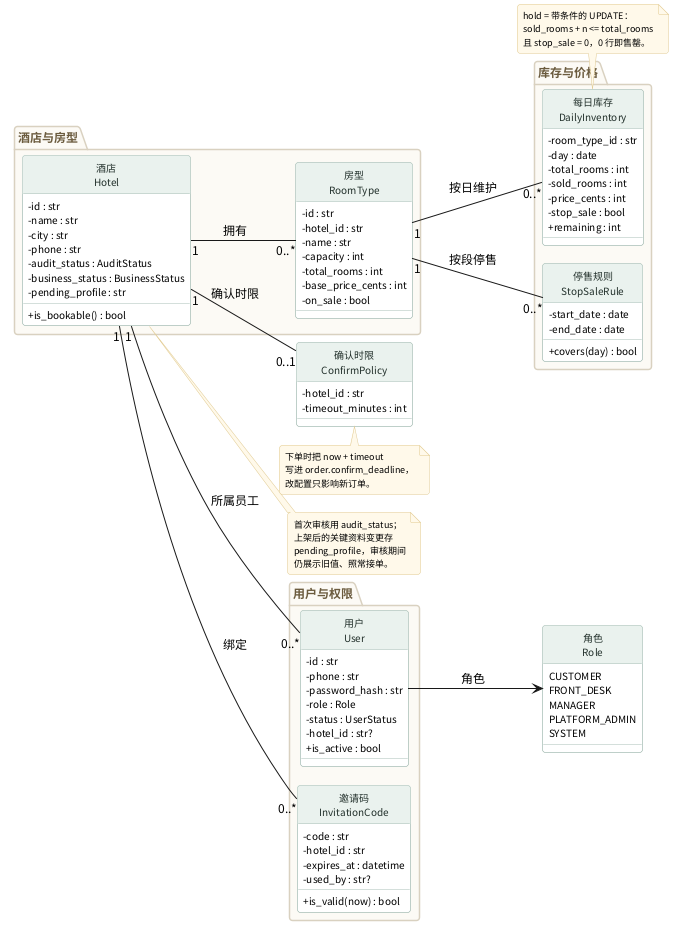
\includegraphics[width=0.72\textwidth]{figs/uml-class-basic.png}
\caption{基础数据类图：用户、酒店、房型、每日库存、停售与确认时限}
\label{fig:uml-class-basic}
\end{figure}

\begin{figure}[H]
\centering
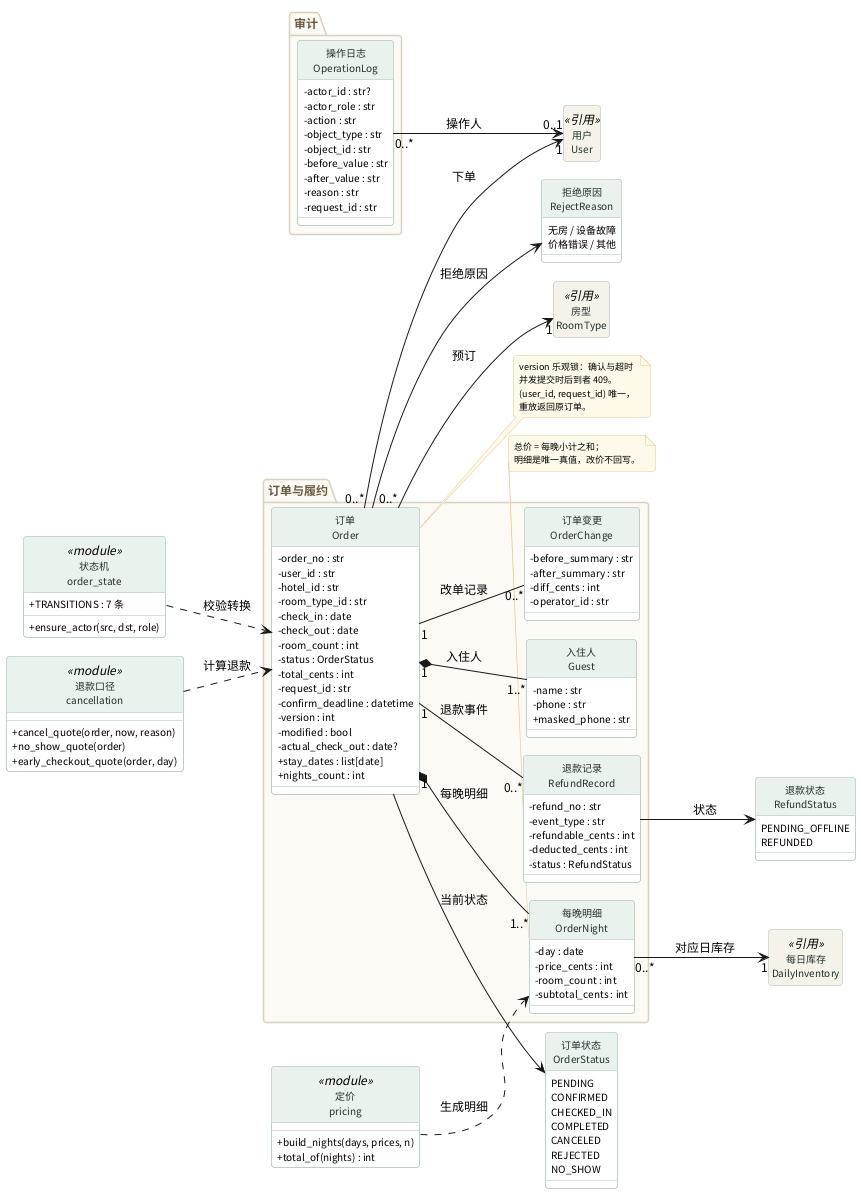
\includegraphics[width=0.78\textwidth]{figs/uml-class-order.png}
\caption{订单与审计类图：订单聚合、退款、变更、日志与状态枚举}
\label{fig:uml-class-order}
\end{figure}

\begin{figure}[H]
\centering
\begin{minipage}{0.54\textwidth}
  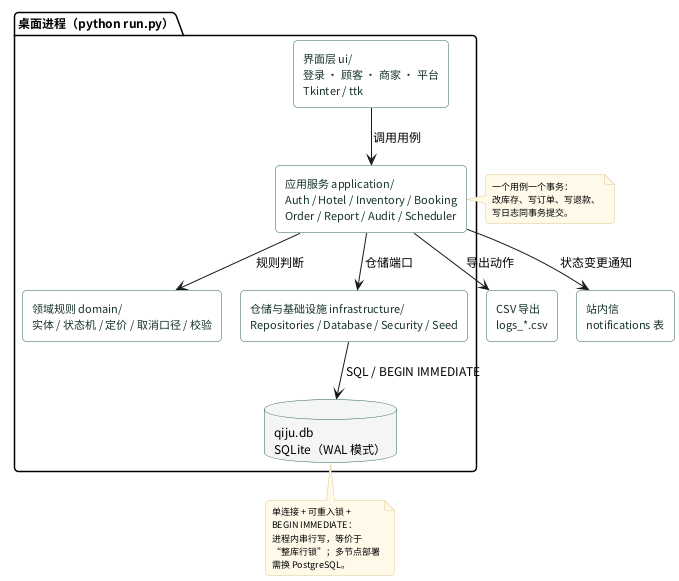
\includegraphics[width=\textwidth]{figs/uml-component.png}
\end{minipage}\hfill
\begin{minipage}{0.42\textwidth}
  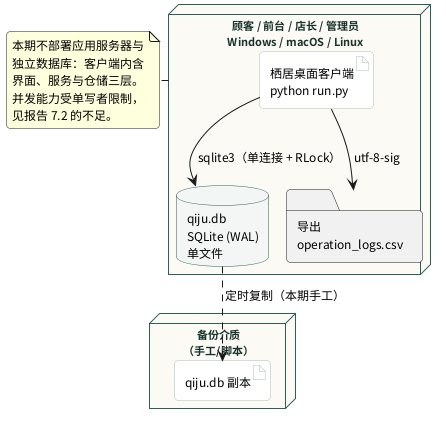
\includegraphics[width=\textwidth]{figs/uml-deploy.png}
\end{minipage}
\caption{组件图与部署图：四层依赖、单机 SQLite、CSV 导出}
\label{fig:uml-deploy}
\end{figure}

% ==================== 2 关键实现 ====================
\section{七个关键实现}

\subsection{金额与日期：把“差不多”变成“一定”}

金额只用整数分，是从实验一就被反复强调的约束（\req{REQ-032}）。实现时我把它变成两条硬规则：实体和表里没有任何 \code{float}；用户输入的“元”只在界面边界转一次分。解析用 \code{Decimal}，并显式检查小数位，避免 \code{19.99 * 100 = 1998.9999...}。

\begin{lstlisting}[style=py]
def parse_yuan(text: str) -> int:
    value = Decimal(text.strip().replace(",", ""))
    if value < 0:
        raise ValueError("金额不能为负")
    if value.as_tuple().exponent < -2:
        raise ValueError("金额最多两位小数")
    return int(value * 100)
\end{lstlisting}

日期统一“入住日含、退房日不含”。订单的 \code{stay_dates} 直接用 \code{range(check_in, check_out)} 生成，库存、明细、改单、对账都复用这一个定义，避免出现“有的地方算 3 晚、有的地方算 2 晚”。

\subsection{逐晚扣减：一条带条件的 UPDATE}

这是整个实现里最不能错的一段。REQ-008 要求“任一晚不足则整单失败”，REQ-029 要求“50 并发抢 1 间只能成功 1 个”。我一开始也写过“先查剩余、再更新”，写完立刻删了：两个请求都读到 1 间、都判断够、都扣，库存就成负数了。最终只保留一条条件 \code{UPDATE}：

\begin{lstlisting}[style=py]
def hold(self, room_type_id: str, day: date, count: int) -> bool:
    cursor = self.db.execute(
        """
        UPDATE daily_inventory
           SET sold_rooms = sold_rooms + ?
         WHERE room_type_id = ? AND day = ?
           AND stop_sale = 0
           AND sold_rooms + ? <= total_rooms
        """,
        (count, room_type_id, day.isoformat(), count),
    )
    return cursor.rowcount == 1
\end{lstlisting}

\code{rowcount == 0} 就是售罄或停售，不需要再查一次。三晚的循环放在同一个 \code{with db.transaction()} 里，任何一晚返回 \code{False} 就抛 \code{SoldOut}，外层回滚，前两晚的扣减不会留下。下单事务的顺序固定为：幂等查重 → 逐晚 \code{ensure}（无记录时按房型默认值建行）→ 逐晚 \code{hold} → 写订单/明细/入住人 → 写日志 → \code{COMMIT}。

并发用例在 \code{tests/test_concurrency.py}：50 个线程、每人独立 \code{request_id}、抢同一晚最后 1 间。结果恰好 1 单成功、49 个 \code{SOLD_OUT}、库存 1、订单 1 张。这个测试不是“跑通就行”，它必须同时断言成功数、库存和异常类型，否则全失败也能通过。

\subsection{状态机：一张表管住 7 个状态}

状态机写成表，而不是一串 \code{if}。每条转换带四样东西：目标状态、允许的角色、是否必须写原因、对库存的影响。服务层只做守卫（库存复核、入住日、18:00），能不能转、谁能转由表回答。

\begin{table}[H]
\centering
\caption{7 条允许转换（与 \code{TRANSITIONS} 一一对应）}
\label{tab:transitions}
\small
\begin{tabularx}{\textwidth}{@{}p{1.7cm}p{1.9cm}p{2.3cm}p{4.1cm}X@{}}
\toprule
当前 & 目标 & 动作 & 角色 & 守卫 / 库存影响 \\
\midrule
待确认 & 已确认 & confirm & 前台、店长 & 库存复核通过；库存不变 \\
待确认 & 已拒绝 & reject & 前台、店长 & 原因四选一，“其他”需说明；释放全部 \\
待确认 & 已取消 & cancel & 顾客、系统 & 顾客取消或确认超时；释放全部 \\
已确认 & 已入住 & check\_in & 前台、店长 & 入住日当天；提前需店长+原因；库存不变 \\
已确认 & 已取消 & cancel & 顾客、前台、店长、管理员、系统 & 18:00 规则/停业/强制；释放全部 \\
已确认 & 未入住关闭 & no\_show & 系统 & 入住日 24:00；释放入住日之后 \\
已入住 & 已完成 & check\_out & 前台、店长 & 正常退房不释放；提前退房需店长 \\
\bottomrule
\end{tabularx}
\end{table}

禁止的转换由 \code{find_transition} 直接抛 409。测试里覆盖了三类典型非法转换：\code{COMPLETED→CANCELED}、\code{PENDING→CHECKED_IN}、\code{CONFIRMED→REJECTED}；另有角色不符（顾客确认）和终态再操作。并发安全靠订单上的 \code{version}：\code{UPDATE ... WHERE id=? AND version=?} 影响 0 行就返回 409，确认与超时同时提交时只有一个能改。

\begin{figure}[H]
\centering
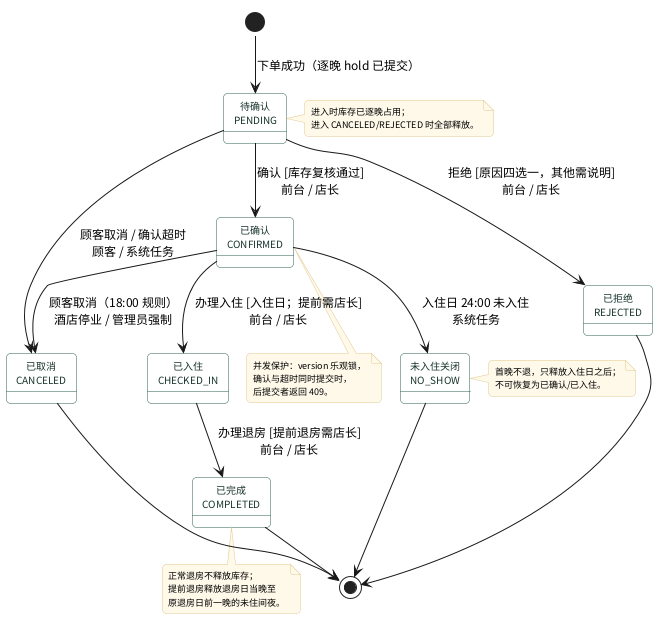
\includegraphics[width=0.62\textwidth]{figs/uml-state.png}
\caption{7 状态与 7 条允许转换；终态不可恢复}
\label{fig:uml-state}
\end{figure}

图 \ref{fig:uml-seq-confirm} 是“确认”和“超时”同时到达时的时序：两者都读到 \code{version=v}，谁先提交谁把 \code{version} 改成 $v+1$，后提交者 \code{UPDATE} 影响 0 行，返回 409。

\begin{figure}[H]
\centering
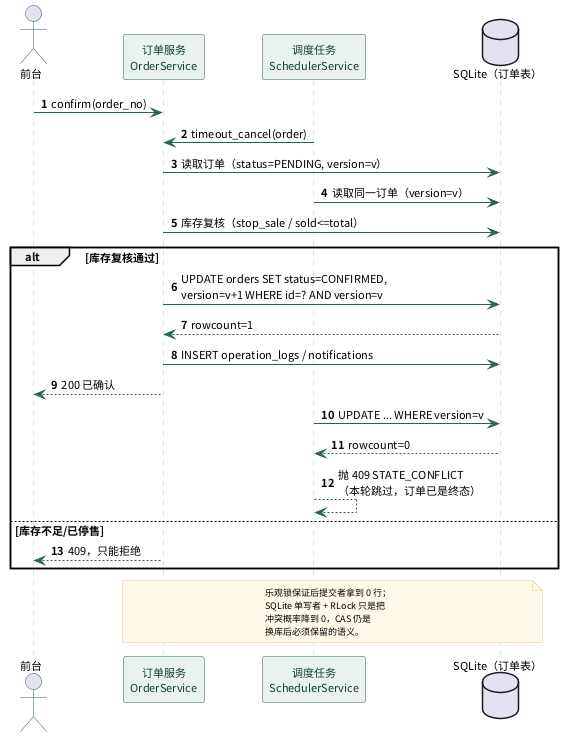
\includegraphics[width=0.55\textwidth]{figs/uml-seq-confirm.png}
\caption{确认与超时并发：乐观锁让后提交者拿到 0 行}
\label{fig:uml-seq-confirm}
\end{figure}

\subsection{幂等与重复下单：唯一键 + 二次确认}

\req{REQ-024} 有两层：同一 \code{request_id} 重放返回原单；不同 \code{request_id} 但 2 分钟内内容相同，要先提示、顾客确认后才建新单。实现分三层：

\begin{itemize}[leftmargin=1.6em,itemsep=1pt,topsep=2pt]
  \item 数据库层：\code{UNIQUE(user_id, request_id)}，并发重放最终只有一条能插入；
  \item 事务层：进入事务后再查一次幂等键，挡住“查的时候还没有、插的时候已经有了”的窗口；
  \item 业务层：查 2 分钟内同酒店、房型、日期、间数、入住人集合的订单，命中就抛 \code{DuplicateOrder}；界面弹“仍然创建”，重提时带 \code{confirm_duplicate=True}。
\end{itemize}

\begin{figure}[H]
\centering
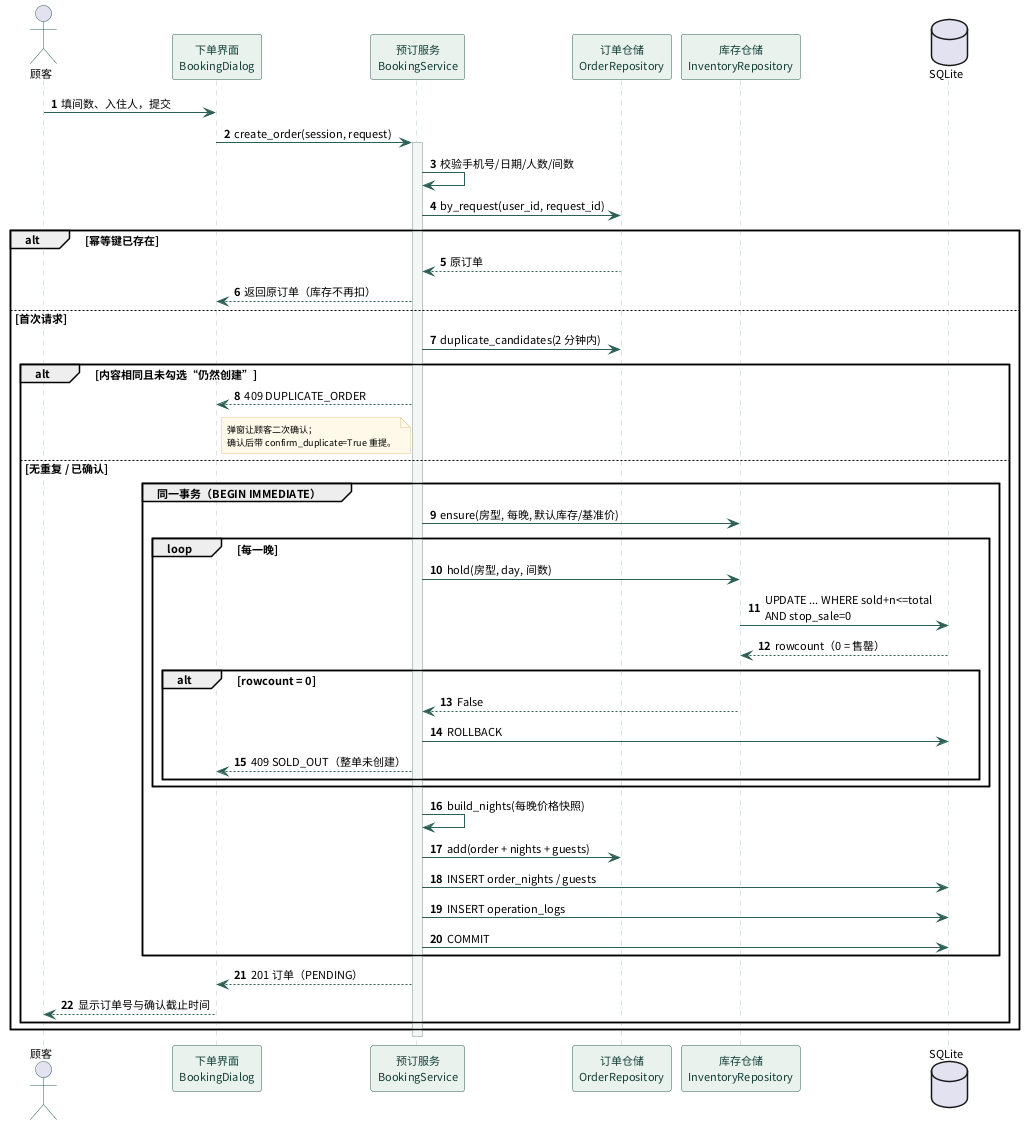
\includegraphics[width=0.82\textwidth]{figs/uml-seq-booking.png}
\caption{提交预订：幂等查重、2 分钟重复确认、逐晚 hold、同事务提交}
\label{fig:uml-seq-booking}
\end{figure}

这里有个容易忽略的细节：比较入住人不能只比人数，要比 \code{(name, phone)} 集合；否则“同一间房换一个入住人”会被误判成重复。窗口的 2 分钟用订单 \code{created_at} 比较，而不是当前时间减 2 分钟再格式化成字符串。

\subsection{退款三口径：18:00、未入住、提前退房}

退款金额由 \code{cancellation.py} 里的三个纯函数算，服务层只负责释放库存和写退款记录。以“3 晚、每晚 300 元”为例：

\begin{table}[H]
\centering
\caption{三种典型退款场景（3 晚 × 300 元 = 900 元）}
\label{tab:refund}
\small
\begin{tabularx}{\textwidth}{@{}p{3.1cm}p{2.2cm}p{2.3cm}p{2.4cm}X@{}}
\toprule
场景 & 扣费 & 应退 & 释放库存 & 说明 \\
\midrule
入住日 17:59:59 取消 & 0 & 900 & 3 晚 & 18:00:00 及之前免费 \\
入住日 18:00:00 取消 & 0 & 900 & 3 晚 & 边界含 18:00:00 本身 \\
入住日 18:00:01 取消 & 300 & 600 & 3 晚 & 收首晚房费 \\
未入住关闭 & 300 & 600 & 第 2、3 晚 & 首晚保留，只释放之后 \\
提前退房（住 1 晚） & 0 & 600 & 第 2、3 晚 & 按实际入住晚数结算 \\
\bottomrule
\end{tabularx}
\end{table}

边界用 \code{datetime.combine(check_in, time(18, 0), tzinfo=HOTEL_TZ)} 比较，不用 \code{now.hour < 18}——后者会把 18:00:00 判成收费。测试用 \code{FixedClock} 钉在三个时刻，不需要真的等到傍晚。未入住关闭只释放 \code{stay_dates[1:]}，提前退房只释放 \code{day >= actual_check_out} 的间夜；这两条都在测试里用具体日期核对过库存。

\subsection{报表：先定口径，再写 SQL}

\req{REQ-018} 的 8 项指标里，“计费间夜”最容易写错。它不等于“所有订单的间夜”：已确认/已入住/已完成算全部入住间夜；未入住关闭只算首晚；18:00 后取消只算首晚；已拒绝、免费取消不算。停售日的可售间夜计 0。

我把口径拆成三个函数：\code{_billable_days}、\code{_stayed_days}、\code{_sellable_nights}，报表按日聚合后再求和。这样“某一天为什么是 2 间夜”可以直接指着函数说，不用在一大段 SQL 里找。退款按退款记录的创建时间归属，净成交 = 成交金额 $-$ 退款金额；除数为 0 时界面显示“—”，不抛 \code{ZeroDivisionError}。

\begin{lstlisting}[style=py]
if order.status in (CONFIRMED, CHECKED_IN, COMPLETED):
    days = set(order.stay_dates)
    if order.status is COMPLETED and order.actual_check_out:
        days = {d for d in days if d < order.actual_check_out}
    return days
if order.status is NO_SHOW:
    return {order.check_in}          # 只计首晚
if order.status is CANCELED:
    late = (order.cancel_reason == CUSTOMER.value
            and order.canceled_at > free_cancel_deadline(order.check_in))
    return {order.check_in} if late else set()
return set()
\end{lstlisting}

\subsection{权限、日志与导出}

权限同时校验“功能权限”和“数据范围”（\req{REQ-002}）：越权写返回 403；跨酒店、跨用户的读统一返回 404，不泄露资源是否存在。实现放在 \code{BaseService.require_*}/\code{resolve_order}，业务方法只写“谁能做”，不重复判权限。

日志与业务同事务：\code{write_log} 在 \code{with db.transaction()} 里调用，业务失败回滚时日志也不落库。13 个字段按 \req{REQ-019} 对齐；手机号在写入前用正则脱敏成“前三位 + **** + 后四位”，导出 CSV 时再走一遍同样的数据。日志仓储只有 \code{add}/\code{query}，没有 \code{update}/\code{delete}。

导出用 \code{utf-8-sig}，Excel 双击不乱码；导出动作本身再写一条 \code{LOG_EXPORT} 日志，否则“谁把日志导走了”查不到。店长只能导本店，管理员可导全平台；越权用 403，不是返回空列表。

\subsection{调度与对账：两个只有跑起来才会发现的 bug}

调度器每 30 秒被界面调一次（\code{after(30000)}，不是主线程 \code{sleep}），做三件事：确认超时、未入住关闭、未来两周对账。它不直接改状态，而是调用订单服务的 \code{timeout_cancel}/\code{close_no_show}，保证退款和日志口径一致。

实现过程中抓到两个 bug，都是测试写出来才发现的：

\begin{enumerate}[leftmargin=1.6em,itemsep=2pt,topsep=2pt]
  \item \textbf{确认时限用了“当前 policy”反推。}第一版 \code{_timeouts} 用 \code{now - policy.timeout} 和 \code{created_at} 比较。测试“改配置只影响新订单”时，旧订单被新 policy 提前取消了。改成订单上的 \code{confirm_deadline} 快照后，测试才过。
  \item \textbf{对账把提前退房释放的间夜又算成占用。}第一版对账把 \code{COMPLETED} 订单的所有间夜都算进“应占用”，提前退房释放掉的那两晚就出现了 1 条差异。查了半小时才定位到 \code{actual_check_out}：对账必须跳过 \code{day >= actual_check_out} 的间夜。
\end{enumerate}

\subsection{界面层：三端十屏与“异常态”}

界面按角色分：顾客 3 屏（搜索/详情/我的订单）、商家 4 屏（工作台、房态、房型、报表）、平台 3 屏（酒店审核、全平台订单、确认时限），外加登录、日志、消息。每个列表页都留了详情栏，避免“点进去再退出来”的来回跳。

异常态是重点：搜索页把售罄和停售分开（停售不返回结果）；下单弹窗对重复订单二次确认；工作台对非法状态只显示可执行按钮；报表除零显示“—”；日志导出后提示条数。截图见 5.5 节。

界面本身踩了两个坑，写在 4.3 节：Tk 的正数字号在 HiDPI 下会翻倍，以及 \code{pack_propagate(False)} 让表格卡片的请求宽度变成 3 px。前者改成负数字号（像素），后者删掉并给 Treeview 列加 \code{minwidth} 和横向滚动条。

% ==================== 3 代码风格与质量 ====================
\section{代码风格、测试与质量}

\subsection{规范与静态检查}

按课程对代码风格的要求，工程用 \code{ruff} 做风格门禁，配置写在 \code{pyproject.toml}：行宽 100，目标 Python 3.10，启用 \code{E/F/W/I/UP/B/SIM/C90}，\code{mccabe} 最大复杂度 14。选择这几组规则的原因很实际：\code{E/F} 抓语法与未使用变量，\code{I} 抓 import 顺序，\code{B} 抓可变默认值等陷阱，\code{SIM} 抓可以简化的分支，\code{C90} 防止一个方法长成“面条”。

交付前运行：

\begin{lstlisting}[language=bash,basicstyle=\ttfamily\footnotesize,frame=single,rulecolor=\color{line},backgroundcolor=\color{paper}]
$ ruff check qiju tests run.py
All checks passed!
\end{lstlisting}

代码里 101 个类、412 个函数，全部带类型注解；公开类与方法有中文 docstring，解释“为什么这样做”，而不是复述“这是什么”。例如 \code{hold} 的 docstring 写的是“条件写在 WHERE 里而不是先查后改，是避免先查后扣的唯一办法”，而不是“占用库存”。

\subsection{测试：97 个用例与 84\% 核心覆盖率}

测试按业务域分 11 个文件，共 97 个用例。核心层（domain + application + infrastructure，排除演示数据）覆盖率 84\%，其中 domain 91\%、application 82\%、infrastructure 85\%。总覆盖率 45\%，因为 3,591 行界面没有自动化测试——这是本实验最大的缺口，写在 7.2。

\begin{table}[H]
\centering
\caption{测试分布}
\label{tab:tests}
\small
\begin{tabularx}{\textwidth}{@{}p{3.6cm}>{\raggedleft\arraybackslash}p{1.2cm}X@{}}
\toprule
测试文件 & 用例数 & 覆盖重点 \\
\midrule
\code{test_domain.py} & 18 & 金额、定价、7 状态、18:00 边界、校验 \\
\code{test_booking.py} & 13 & 下单、快照、售罄回滚、幂等、重复确认 \\
\code{test_concurrency.py} & 1 & 50 线程抢 1 间房 \\
\code{test_orders.py} & 15 & 确认/拒绝/取消/入住/退房/退款/强制取消 \\
\code{test_modify.py} & 7 & 重叠日期、失败原单不变、只改一次 \\
\code{test_inventory.py} & 9 & 单日/批量、停售跳过、低于已售拒绝 \\
\code{test_reports.py} & 4 & no-show、18:00 后取消、口径与除零 \\
\code{test_scheduler.py} & 5 & 超时、未入住、对账漂移、通知脱敏 \\
\code{test_permissions.py} & 10 & 403/404、跨酒店、停用账号、登录提示 \\
\code{test_audit.py} & 9 & 同事务、脱敏、导出、乐观锁 \\
\code{test_hotels.py} & 6 & 入驻审核、邀请码、资料变更、停业 \\
\midrule
合计 & 97 & \code{pytest} 0.65 秒跑完 \\
\bottomrule
\end{tabularx}
\end{table}

测试里最值钱的是三类“反例”：售罄时前两晚必须回滚、改单失败时原单和库存不能变、未入住关闭后首晚库存必须还在。这三类用例抓到的 bug 比正常路径多得多。

\subsection{一次自查：把“看起来对”改成“算得对”}

交付前我按 \code{chat.txt} 的 CHK 清单逐项过，发现两处不是“代码错了”，而是“口径错了”：

\begin{itemize}[leftmargin=1.6em,itemsep=1pt,topsep=2pt]
  \item 报表最初把 no-show 订单的全部间夜计入成交额，导致 2 晚 596 元的 no-show 订单报表显示 596 元成交，而 \req{REQ-018} 只允许首晚 298 元。改成 \code{_billable_days} 后，测试里的 3 晚 900 元 no-show 只计 300 元。
  \item 对账最初把提前退房释放的间夜算成“应占用”，出现 1 条假差异。修正后，\code{test_scheduler.py} 里的对账用例 只有在真正多扣库存时才会报差异。
\end{itemize}

这两处都不是语法错误，静态检查也抓不到；只能靠“拿需求表逐项对 + 用具体数字手算”发现。这也是我后来越来越依赖测试的原因：它逼我把“我觉得”写成“我断言”。

% ==================== 4 大模型辅助 ====================
\section{大模型辅助实现的过程与反思}

\subsection{使用原则：让 AI 写“可被检查的代码”}

实验三明确要求用大模型辅助开发，但也要求“阅读并检查每一行即将应用的代码”。我给自己定了三条规矩：

\begin{enumerate}[leftmargin=1.6em,itemsep=2pt,topsep=2pt]
  \item \textbf{先写规约，再让它写实现。}每次不是直接说“写一个下单服务”，而是先给出输入、输出、异常、事务边界和验收用例，再让它填。比如库存扣减，我会写“任一晚失败必须整单回滚；并发下 stock 不得为负；用条件 UPDATE，不许先查后扣”。
  \item \textbf{一次只让它做一件事。}先生成实体和 schema，确认字段与约束；再生成仓储；最后生成服务。一次生成 800 行，看起来快，实际 review 成本更高。
  \item \textbf{它给的每一段 SQL、每一个边界条件，都要有测试。}AI 最容易在“<= 还是 <”“释放全部还是释放之后”“事务里还是事务外”这三类地方出错，而这些恰好都能写成断言。
\end{enumerate}

完整记录在 \code{chat.txt}，按 \code{AI-01}～\code{AI-10} 编号、逐行编号；本节引用行号，例如 \code{AI-03-L008}。

\subsection{十次使用记录汇总}

\begin{table}[H]
\centering
\caption{大模型使用记录汇总（详见 \code{chat.txt}）}
\label{tab:ai-log}
\footnotesize
\begin{tabularx}{\textwidth}{@{}p{0.85cm}p{2.8cm}p{3.7cm}p{4.2cm}p{3.0cm}@{}}
\toprule
编号 & 场景 & 生成结果 & 主要问题 & 人工修订 \\
\midrule
AI-01 & 工程骨架 & 12 个平铺文件，服务里拼 SQL & 无分层、不可测 & 四层 + 仓储门面 \\
AI-02 & 实体与建表 & 金额 float、明细存 JSON & 违反 REQ-032/028 & 整数分、独立明细表、唯一约束 \\
AI-03 & 库存扣减 & 先 SELECT 再 UPDATE & TOCTOU、失败不回滚 & 条件 UPDATE + 事务 \\
AI-04 & 状态机 & 8 条转换，含“完成→取消” & 非法转换、漏 NO\_SHOW & 按表重写 7 条 + 角色/守卫 \\
AI-05 & 退款口径 & 18:00 用 \code{hour<18}；no-show 全退 & 边界错、释放范围错 & 三个纯函数 + 三点测试 \\
AI-06 & 幂等 & 用 order\_no；窗口 2 小时 & 键错、无唯一约束 & (user, request\_id) + 二次确认 \\
AI-07 & 报表 & 总价求和当成交额 & 8 项口径全偏 & 三个口径函数 + 手算对拍 \\
AI-08 & Tkinter & 单文件 900 行、正数字号 & 列被压缩、DPI 失控 & 拆 8 文件、负数字号、after 定时 \\
AI-09 & 测试 & 10 线程、共用 request\_id & 测不到并发、断言太弱 & 50 线程、独立键、断言库存 \\
AI-10 & 报告润色 & 编造“日均 10 万单” & 数字不可回溯 & 删除，改为命令输出 \\
\bottomrule
\end{tabularx}
\end{table}

\subsection{四个典型翻车案例}

\subsubsection{库存：它给的是“先查后扣”}

第一版生成的是 \code{SELECT remaining} → \code{if remaining >= n} → \code{UPDATE sold = sold + n}（\code{AI-03-L004}～\code{L006}）。这段代码在单线程演示里永远是对的，所以我差点留下。后来写到并发测试才反应过来：两个线程同时读到 1 间，都判断“够”，都扣，最后 \code{sold=2}、\code{total=1}。更隐蔽的是失败分支只 \code{return False}，前两晚的扣减已经提交，订单却没创建。

改成条件 \code{UPDATE} 后，逻辑从“查询—判断—写入”三步变成一步，“够不够”由数据库在更新时判断。这个改动的价值不在于 SQL 写法，而在于把并发正确性从“调用方记得加锁”变成“语句本身不可能超卖”。

\subsubsection{状态机：它按“业务常识”补了一条非法转换}

生成的表里有 \code{COMPLETED -> CANCELED}，理由是“客人投诉可以撤销”（\code{AI-04-L003}）。这条在业务讨论里听起来合理，但 \req{REQ-017} 表 4 明确禁止：已完成是终态，取消会破坏收入和库存统计。它还漏了 \code{NO_SHOW}，并且所有转换都没有守卫和角色。

我按需求表重写了 7 条，每条补 \code{actors}、\code{reason_required}、\code{inventory_effect}，再用 \code{ensure_actor} 同时校验“状态”和“角色”。这件事让我记住：AI 的“业务常识”来自它见过的系统，不是来自本项目的需求约定；终态、非法转换、角色矩阵这三类，必须人对着需求表逐行核。

\subsubsection{退款：18:00 的边界错了 1 秒}

生成的是 \code{if now.hour < 18: free}（\code{AI-05-L004}）。这会把 18:00:00 判成收费，而 \req{REQ-012} 写的是“18:00:00 及之前免费，18:00:01 起收费”。1 秒的差别，在真实系统里就是一次客诉。

我改成 \code{now <= datetime.combine(check_in, time(18, 0))}，并把测试钉在 17:59:59、18:00:00、18:00:01 三个时刻。另一个错误是 no-show “全额退款、释放全部库存”；实际是首晚照收、只释放入住日之后。这两个错误都不是“代码写得丑”，而是“规则理解错”，只能靠把需求原文贴在旁边逐字对。

\subsubsection{界面：字号和列宽把布局搞崩了}

Tkinter 的正数字号是“磅”，在 X11/HiDPI 下同一份代码在 96 dpi 和 192 dpi 上能差一倍；我第一版截图里 10 pt 正文实际渲染成 39 px 行高，表格列全被挤扁。改成负数字号（像素）后，截图和真机一致。

另一个坑是 \code{pack_propagate(False)}：我为了让卡片不被表格撑大，把它加在表格卡片的 \code{body} 上，结果卡片的请求宽度变成 3 px，Grid 把 3/5 的空间全给了右侧详情栏，表格列被压到 433 px。删掉这行、给 Treeview 列加 \code{minwidth} 和横向滚动条后，1440 宽下 7 列才完整。这两个问题都不是“AI 不会写界面”，而是“Tk 的布局/字体模型要在真实屏幕上跑一遍才知道”。

\subsection{人工审查清单}

\begin{table}[H]
\centering
\caption{交付前的人工审查（CHK-01～CHK-16）}
\label{tab:checklist}
\footnotesize
\begin{tabularx}{\textwidth}{@{}p{1.25cm}p{6.7cm}p{1.5cm}X@{}}
\toprule
编号 & 检查项 & 结果 & 依据 / 修订 \\
\midrule
CHK-01 & 金额是否全部整数分、是否有 float & 通过 & 实体与 schema 均 int cents \\
CHK-02 & 日期是否左闭右开、退房日是否不计库存 & 通过 & \code{stay_dates} 统一生成 \\
CHK-03 & 逐晚扣减是否原子、失败是否整单回滚 & 通过 & 条件 UPDATE + 事务 + 50 线程 \\
CHK-04 & 是否 7 个状态、是否存在禁止转换 & 通过 & 7 条表 + 禁止转换用例 \\
CHK-05 & 确认前是否复核库存、停售是否只能拒绝 & 通过 & \code{_assert_stock_confirmable} \\
CHK-06 & 18:00 边界是否 18:00:00 免费、18:00:01 收费 & 通过 & FixedClock 三点用例 \\
CHK-07 & 未入住是否只释放首晚之后、首晚是否保留 & 通过 & \code{stay_dates[1:]} \\
CHK-08 & 提前退房是否只释放未住间夜、是否需店长 & 通过 & \code{release_days_after} \\
CHK-09 & 幂等键是否 (user, request\_id) 且有唯一约束 & 通过 & schema UNIQUE + 事务内二次查 \\
CHK-10 & 2 分钟重复是否含入住人比较、可否二次确认 & 通过 & guest 集合 + \code{confirm_duplicate} \\
CHK-11 & 越权是否 403/404、跨酒店是否不泄露存在性 & 通过 & \code{resolve_order} + NotFound \\
CHK-12 & 日志是否与业务同事务、手机号是否脱敏 & 通过 & \code{write_log} + \code{mask_phone} \\
CHK-13 & 报表 8 项口径是否与 REQ-018 一致 & 通过 & no-show/迟到取消手算对拍 \\
CHK-14 & 定时任务是否可拨时钟、重复执行是否安全 & 通过 & \code{FixedClock} + 幂等状态检查 \\
CHK-15 & 密码是否非明文、失败提示是否不泄露账号 & 部分 & PBKDF2 替代 bcrypt，见 7.2 \\
CHK-16 & 报告数字是否可回溯、是否无编造 & 通过 & 行数/覆盖率/测试数均来自命令 \\
\bottomrule
\end{tabularx}
\end{table}

\subsection{哪些环节真的省时间，哪些不能交}

\textbf{省时间的：}（1） 样板代码，比如 dataclass、SQL 建表、CRUD 仓储、Tkinter 的 grid/pack 骨架；（2） 命名和文案，类名、错误提示、按钮文案，它给的比我翻词典快；（3） 检查清单，问“对照 REQ-017 还缺什么”，它能列出漏掉的 NO\_SHOW、超时、幂等点，虽然不保证全对，但比空白页强；（4） 测试骨架，fixture、参数化、断言结构，省掉大量重复。

\textbf{不能交的：}（1） 业务规则的边界（18:00、24:00、首晚、释放范围）；（2） 并发与事务方案（先查后扣、锁的粒度、回滚）；（3） 状态机的允许/禁止转换；（4） 金额与日期口径；（5） 任何要写进报告的数字。判断标准很简单：\emph{这条错了，系统会不会在真实场景里出错？}会，就人来定，AI 只做实现。

\subsection{体会}

这次最大的变化不是“写得更快”，而是“review 的方式变了”。以前我看 AI 代码主要看能不能跑；现在我优先看三件事：SQL 有没有把条件写进 \code{WHERE}、状态转换有没有对需求表、金额和日期有没有用错类型。这三件事一旦对了，剩下的命名和格式反而是小事。

另一个体会是：AI 很擅长把“错的东西写得很整齐”。一张排版漂亮的类图、一段缩进完美的 \code{SELECT} + \code{UPDATE}，比手写的乱代码更危险，因为它看起来可信。人最有价值的工作不是改语法，而是守住那几条不能错的规则，并且用测试把它们钉住。

% ==================== 5 编译、运行与结果 ====================
\section{编译、运行与结果}

\subsection{环境与构建}

运行环境是 Ubuntu 24.04、Python 3.12.3、Tk 8.6、SQLite 3.45.1。运行时没有第三方依赖；开发工具只有 pytest 9.1.1、pytest-cov 与 ruff 0.17.3。Python 没有单独的编译步骤，构建就是“建虚拟环境、装开发工具、做一次字节码编译检查、直接运行”：

\begin{lstlisting}[language=bash,basicstyle=\ttfamily\footnotesize,frame=single,rulecolor=\color{line},backgroundcolor=\color{paper}]
$ cd code
$ python -m venv .venv && . .venv/bin/activate
$ pip install -e ".[dev]"
$ python -m compileall -q qiju && echo "compile ok"
$ python run.py --db ./qiju.db          # 启动桌面端
$ python -m qiju.cli demo               # 无界面跑主流程
$ python -m pytest                      # 97 passed
$ ruff check qiju tests run.py          # All checks passed!
\end{lstlisting}

首次启动会在数据库里写入两段演示数据：一段是十天前的历史订单（已完成、提前退房、18:00 后取消、未入住关闭），一段是今天工作台上的待确认/已确认/已入住订单。这样报表、日志、工作台截图都不是空表，也不需要手工改库。

\subsection{命令行主流程的实际输出}

\code{python -m qiju.cli demo} 用内存库把“查询 → 下单 → 幂等 → 确认 → 入住 → 退房 → 异常分支 → 报表”跑一遍。下面是原样输出（订单号是随机生成的，每次不同）：

\begin{tcolorbox}[enhanced, breakable, colback=paper, colframe=line, boxrule=0.4pt,
  left=8pt, right=8pt, top=6pt, bottom=6pt, arc=2pt, fontupper=\ttfamily\scriptsize]
\begin{verbatim}
======== 1. 可订查询 ========
  栖居·夫子庙店      庭院双床房    2 晚 合计   ¥756.00 剩余 8 间
  栖居·夫子庙店      河景大床房    2 晚 合计   ¥816.00 剩余 11 间
  栖居·新街口店      商务双床房    2 晚 合计   ¥836.00 剩余 16 间
  栖居·新街口店      城景大床房    2 晚 合计   ¥896.00 剩余 20 间

======== 2. 提交预订（逐晚扣减 + 幂等） ========
  订单号 QJ20261030747913，状态 PENDING，总价 ¥756.00
  同一 request_id 重放返回同一订单：True
  重复内容提示：2 分钟内已有相同订单，请确认是否重复提交
    2026-10-31  ¥378.00 × 1
    2026-11-01  ¥378.00 × 1

======== 3. 确认 → 入住 → 退房 ========
  最终状态 COMPLETED，退款记录 0 条

======== 4. 异常分支 ========
  超卖拦截：2026-10-31 库存不足，整单未创建
  非法状态转换：不允许的状态转换：COMPLETED → CONFIRMED

======== 5. 定时任务与对账 ========
  超时取消 0 张，未入住关闭 0 张，对账差异 0 条

======== 6. 经营报表（最近 14 天） ========
  可售 364 间夜，计费 10 间夜，已住 6 间夜
  出租率 2.7%，平均房价 ¥387.00，成交 ¥3870.00，退款 ¥1272.00
  演示账号：13600000001 / Qiju@2026
\end{verbatim}
\end{tcolorbox}

\subsection{走查场景与结果}

除了命令行，我还按 \req{REQ-017}、\req{REQ-029} 的验收方法在测试里跑了下面这些场景。表 \ref{tab:walkthrough} 的“实际结果”都来自测试断言，不是手填的：

\begin{table}[H]
\centering
\caption{关键场景走查（对应测试文件）}
\label{tab:walkthrough}
\footnotesize
\begin{tabularx}{\textwidth}{@{}p{3.4cm}p{4.2cm}Xp{3.1cm}@{}}
\toprule
场景 & 操作 & 实际结果 & 用例 \\
\midrule
主流程 & 搜索 2 晚 → 下单 → 确认 → 入住 → 正常退房 & 状态 COMPLETED；库存不释放；退款 0 条 & \code{test_orders} \\
幂等重放 & 同一 \code{request_id} 连发两次 & 返回同一订单 id；库存只扣 1 次 & \code{test_booking} \\
重复内容 & 2 分钟内不同 \code{request_id}、同内容 & 409 \code{DUPLICATE_ORDER}；确认后建第二单 & \code{test_booking} \\
售罄回滚 & 2 间房订 2 间，第二晚只剩 1 间 & \code{SOLD_OUT}；第一晚库存仍为 0 & \code{test_booking} \\
18:00 取消 & 入住日 18:00:01 取消 & 扣首晚 300；应退 600；释放 3 晚 & \code{test_orders} \\
未入住关闭 & 入住日次日 00:10 跑调度 & NO\_SHOW；首晚仍占；第 2 晚释放 & \code{test_scheduler} \\
提前退房 & 3 晚订单住 1 晚，店长退房 & 释放第 2、3 晚；应退 600；前台单独操作 403 & \code{test_orders} \\
50 并发 & 50 线程抢 1 间房 & 恰好 1 单成功、49 个 \code{SOLD_OUT}、库存 1 & \code{test_concurrency} \\
跨店越权 & 店长 B 查店长 A 的订单 & 404（不泄露存在性） & \code{test_permissions} \\
日志导出 & 店长导出本店 CSV & 手机号脱敏；多一条 \code{LOG_EXPORT} 日志 & \code{test_audit} \\
\bottomrule
\end{tabularx}
\end{table}

\subsection{测试与覆盖率}

\begin{tcolorbox}[enhanced, breakable, colback=paper, colframe=line, boxrule=0.4pt,
  left=8pt, right=8pt, top=6pt, bottom=6pt, arc=2pt, fontupper=\ttfamily\footnotesize]
\begin{verbatim}
$ python -m pytest
........................................................................ [ 74%]
.........................                                                [100%]
97 passed in 0.65s
\end{verbatim}
\end{tcolorbox}

\begin{table}[H]
\centering
\caption{覆盖率（\code{pytest --cov=qiju}；核心层不含 \code{seed.py}）}
\label{tab:coverage}
\small
\begin{tabularx}{\textwidth}{@{}p{4.4cm}>{\raggedleft\arraybackslash}p{1.8cm}>{\raggedleft\arraybackslash}p{1.8cm}X@{}}
\toprule
范围 & 语句数 & 覆盖率 & 说明 \\
\midrule
\code{domain/} & 539 & 91\% & 实体、状态机、退款口径、校验 \\
\code{application/} & 1{,}225 & 82\% & 预订、履约、库存、报表、调度、审计 \\
\code{infrastructure/}（不含 seed） & 442 & 85\% & SQLite、仓储、映射、口令 \\
核心层合计 & 2{,}206 & 84\% & 业务规则与数据访问 \\
全部（含 UI 与 seed） & 4{,}261 & 45\% & UI 层 3{,}591 行未做自动化测试 \\
\bottomrule
\end{tabularx}
\end{table}

界面层没有自动化测试，这是有意取舍：Tkinter 的控件断言成本高、收益低，我把有限的时间放在“金额/库存/状态”这些错了会出事的规则上。界面用 \code{scripts/capture_ui.py} 逐页打开、逐页截图，至少保证 10 屏不会在运行时抛异常；但“按钮点下去之后的交互”没有回归测试，写在不足里。

\subsection{界面截图}

图 \ref{fig:ui-login} 到图 \ref{fig:ui-logs} 是实际运行截图（1440$\times$900，ImageMagick 抓取 X11 窗口），不是设计稿。为了让读者看清，登录与搜索、下单与工作台、房态与报表、审核与日志分成四组。

\begin{figure}[H]
\centering
\begin{minipage}{0.49\textwidth}
  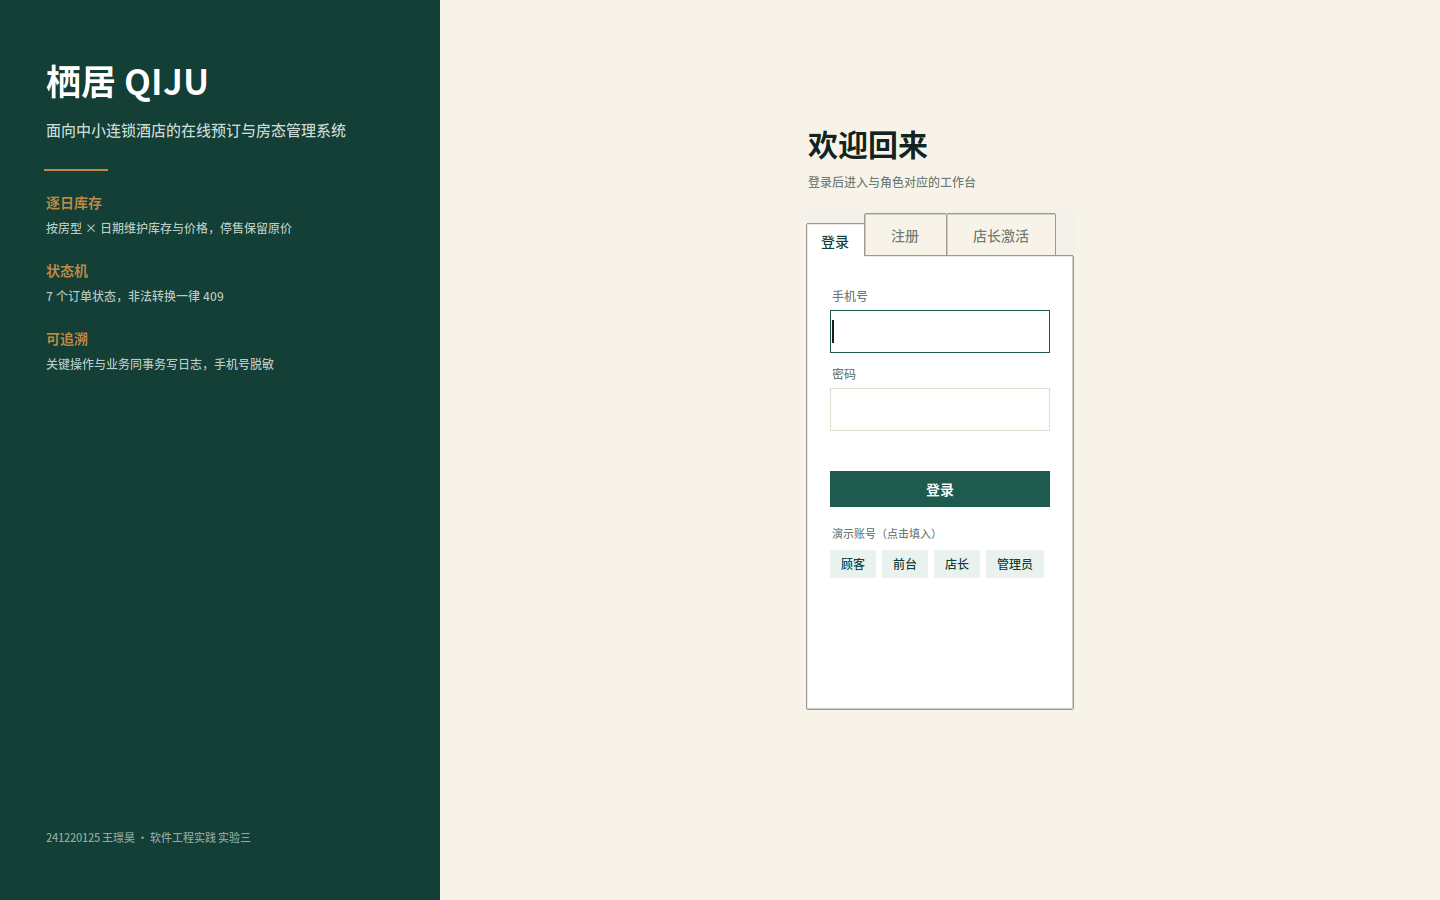
\includegraphics[width=\textwidth]{figs/ui-01-login.png}
\end{minipage}\hfill
\begin{minipage}{0.49\textwidth}
  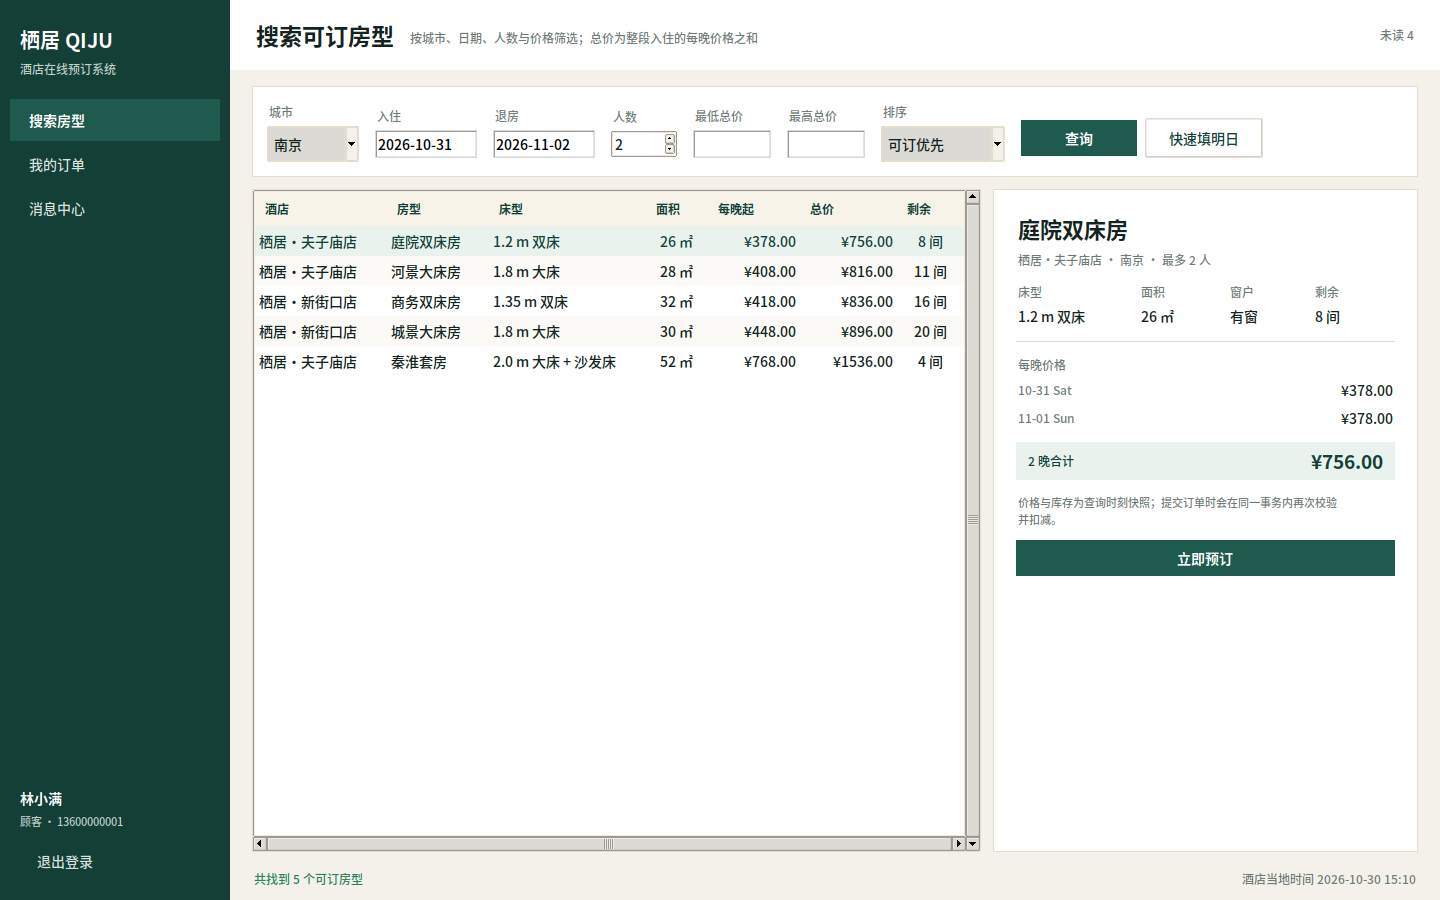
\includegraphics[width=\textwidth]{figs/ui-02-search.png}
\end{minipage}
\caption{登录页与顾客搜索页：搜索结果、每晚价格与剩余间数}
\label{fig:ui-login}
\end{figure}

\begin{figure}[H]
\centering
\begin{minipage}[c]{0.36\textwidth}
  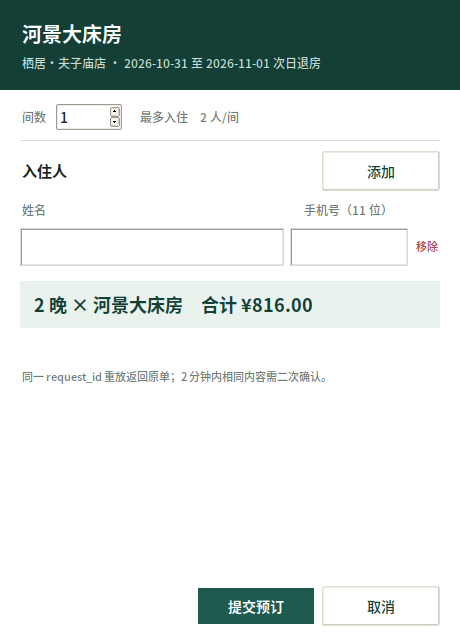
\includegraphics[width=\textwidth]{figs/ui-04-booking-dialog.png}
\end{minipage}\hfill
\begin{minipage}[c]{0.60\textwidth}
  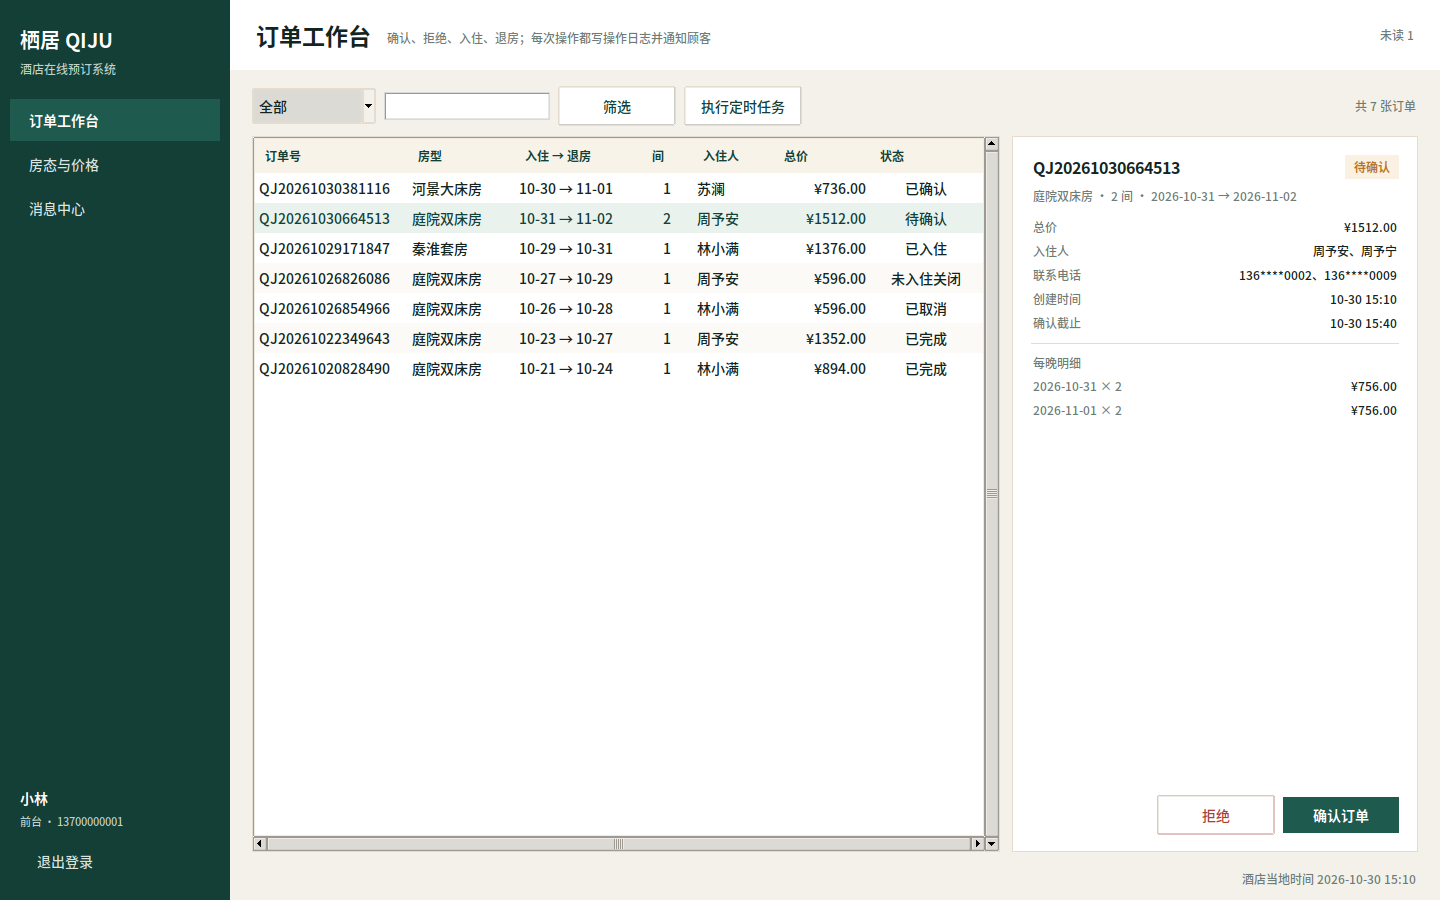
\includegraphics[width=\textwidth]{figs/ui-06-workbench.png}
\end{minipage}
\caption{填写入住人与订单工作台：待确认订单的确认/拒绝入口}
\label{fig:ui-workbench}
\end{figure}

\begin{figure}[H]
\centering
\begin{minipage}{0.49\textwidth}
  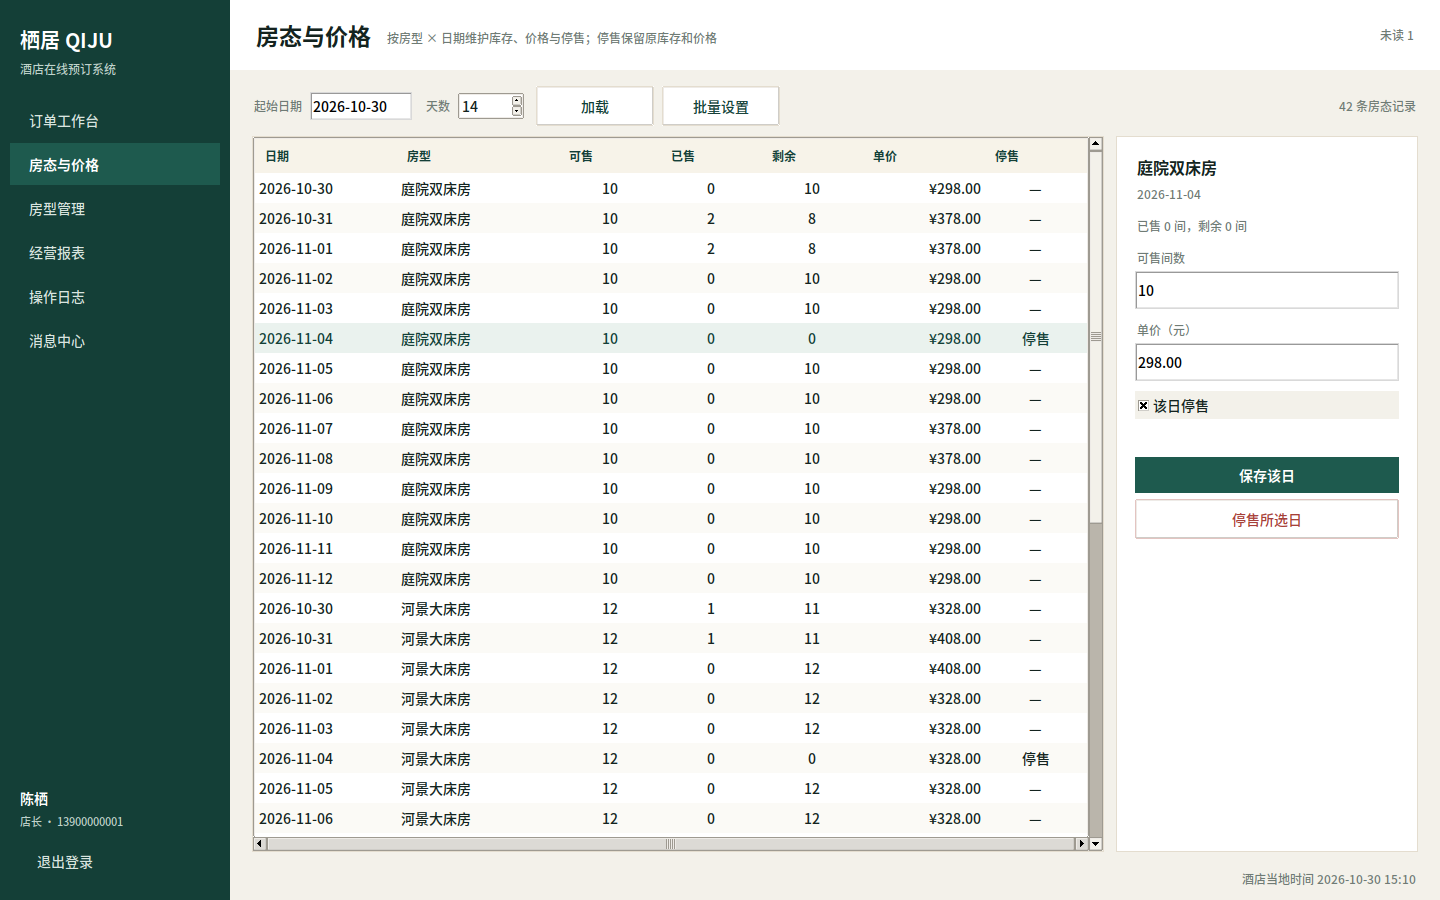
\includegraphics[width=\textwidth]{figs/ui-07-calendar.png}
\end{minipage}\hfill
\begin{minipage}{0.49\textwidth}
  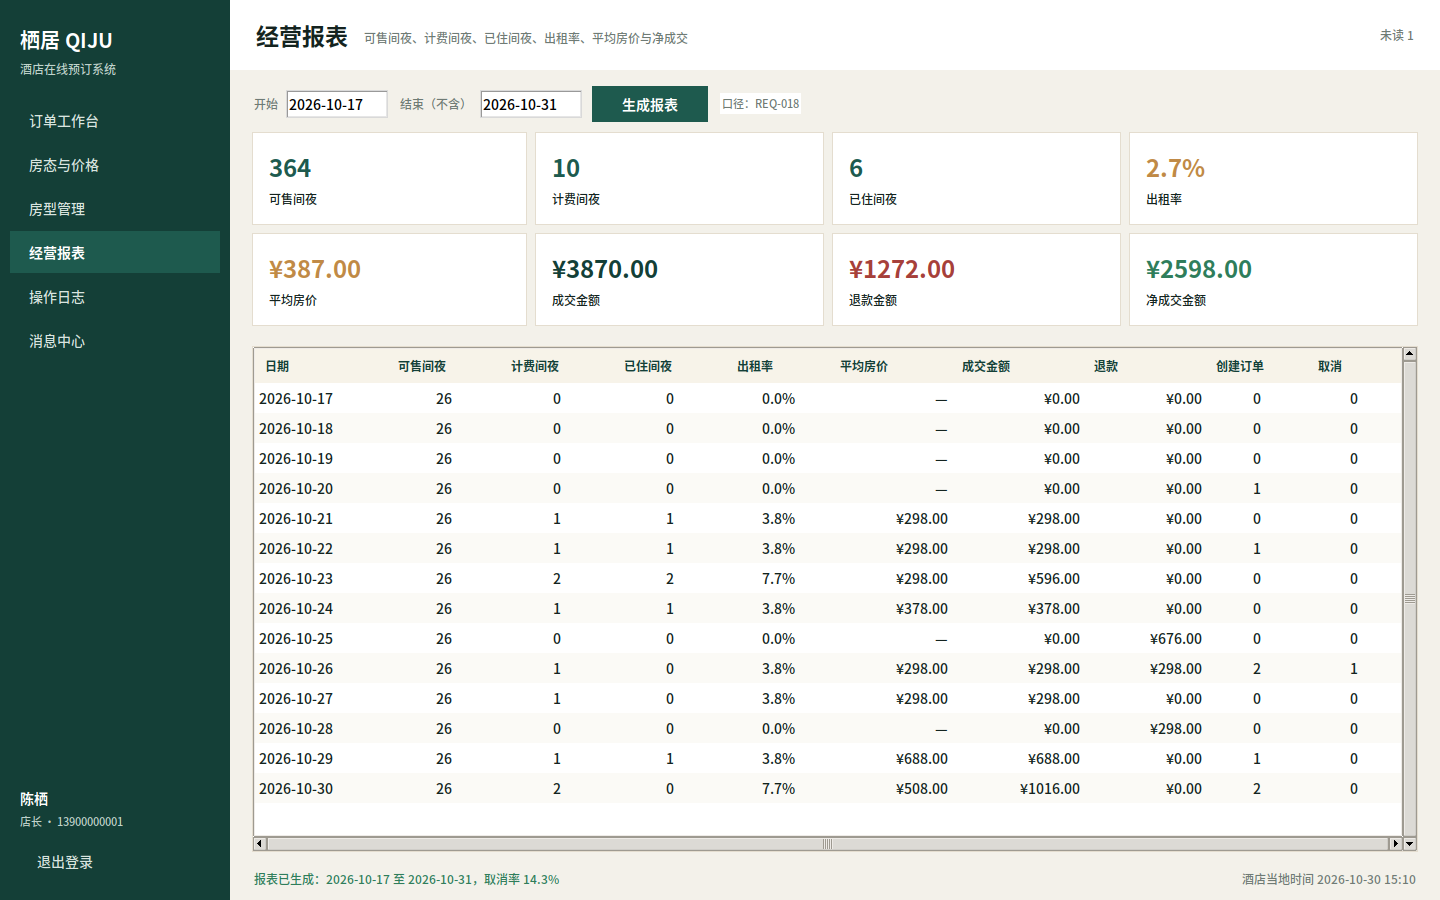
\includegraphics[width=\textwidth]{figs/ui-08-report.png}
\end{minipage}
\caption{房态与价格（含停售日）与经营报表（8 项指标 + 按日明细）}
\label{fig:ui-report}
\end{figure}

\begin{figure}[H]
\centering
\begin{minipage}{0.49\textwidth}
  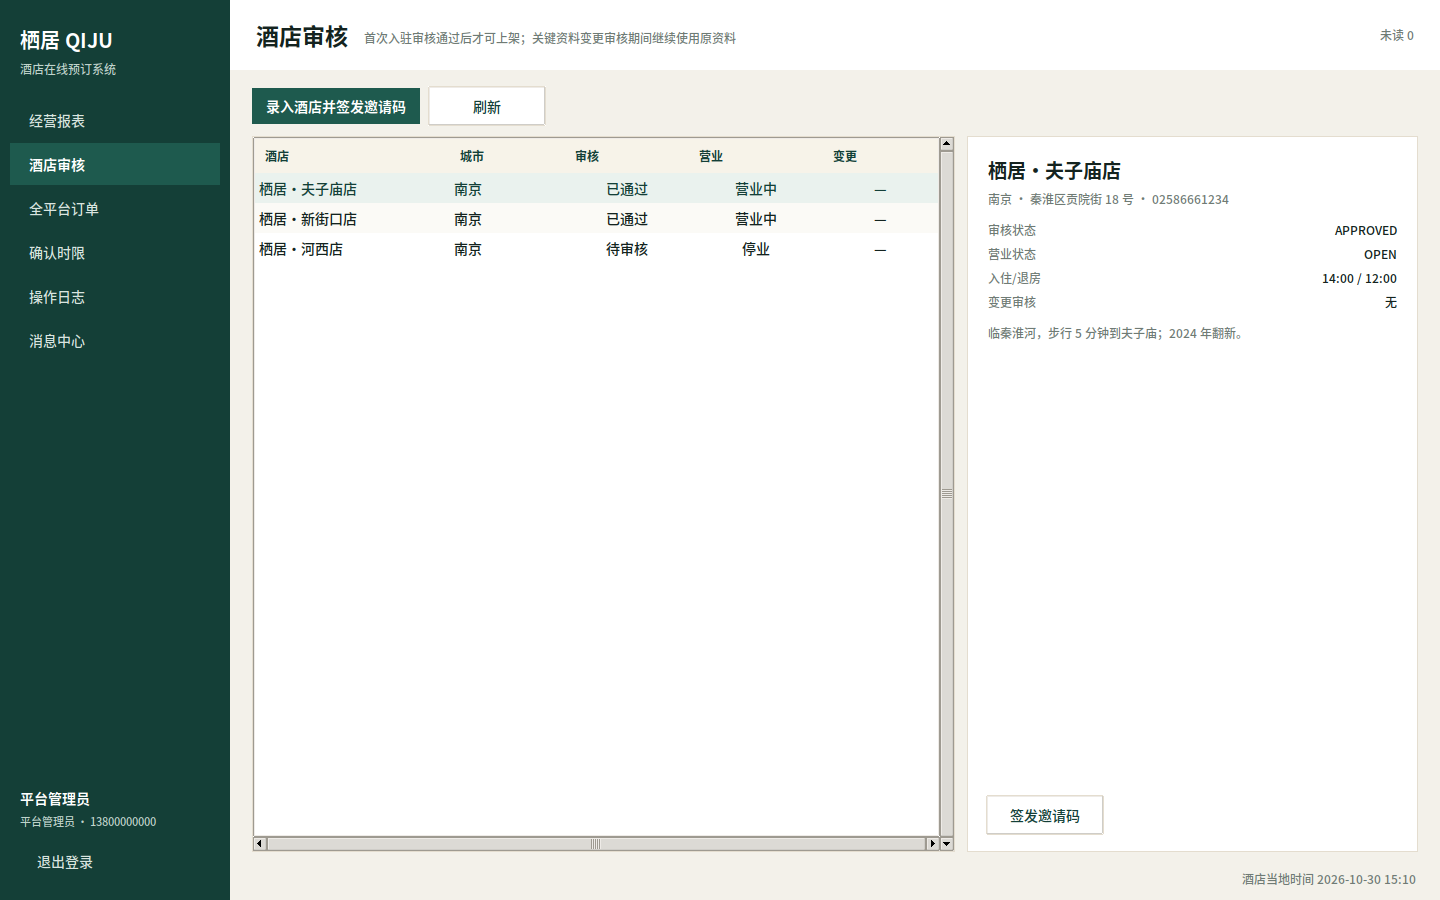
\includegraphics[width=\textwidth]{figs/ui-09-hotel-audit.png}
\end{minipage}\hfill
\begin{minipage}{0.49\textwidth}
  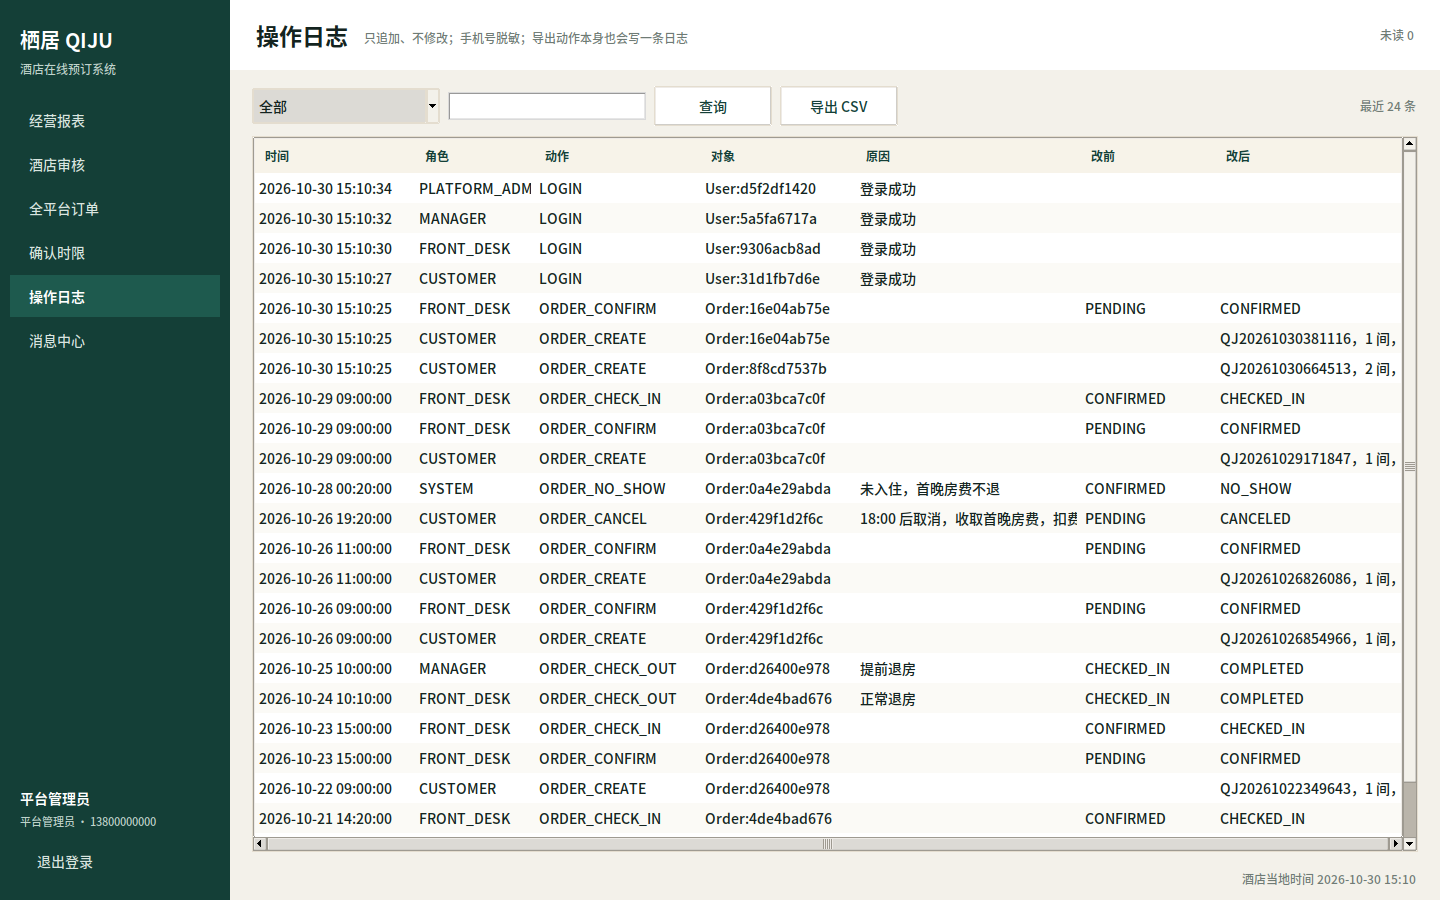
\includegraphics[width=\textwidth]{figs/ui-10-logs.png}
\end{minipage}
\caption{平台端酒店审核与操作日志（手机号已脱敏）}
\label{fig:ui-logs}
\end{figure}

\subsection{运行时才发现的问题}

有三个问题在静态检查里完全看不出来，只有真正启动窗口、拖动列宽、切换页面才暴露：

\begin{enumerate}[leftmargin=1.6em,itemsep=2pt,topsep=2pt]
  \item \textbf{字号单位。}Tk 的正数字号是“磅”，在 HiDPI 下 \code{10} 能渲染成 39 px 行高，表格列全被挤扁；改成负数字号（像素）后，截图和真机一致。
  \item \textbf{Grid 的请求宽度。}\code{pack_propagate(False)} 让表格卡片的请求宽度变成 3 px，Grid 把 3/5 的空间分给右栏；删掉后左表才拿到 672 px，7 列完整。
  \item \textbf{演示数据的时钟。}最初 \code{seed_demo} 在服务构造后替换 \code{ctx.clock}，服务里缓存的 \code{self.clock} 不跟着变，历史订单的时间全错。改成 \code{BaseService.clock} 属性实时读容器，测试和演示数据才一致。
\end{enumerate}

% ==================== 6 Git ====================
\section{Git 本地与远程仓库}

\subsection{仓库与目录}

实现仓库为 \href{https://github.com/aierfula-max/lab3-implementation-241220125}{github.com/aierfula-max/lab3-implementation-241220125}，分支 \code{main}。仓库根目录就是压缩包解压后的目录，报告、UML、代码、AI 记录放在一起，评审不需要在多个仓库之间跳。

\begin{keybox}[仓库结构]
\small
\begin{itemize}[leftmargin=1.4em,itemsep=1pt,topsep=1pt]
  \item \code{实验报告.pdf} / \code{实验报告.tex}：报告与源文件
  \item \code{UML/}：7 组 \code{.puml} 与 \code{.png}
  \item \code{code/}：\code{qiju/}（四层）、\code{tests/}（97 例）、\code{run.py}、\code{scripts/}
  \item \code{chat.txt}：AI-01～AI-10、CHK-01～CHK-16
  \item \code{report/figs/}：报告引用的 UML 与界面截图
\end{itemize}
\end{keybox}

\code{.gitignore} 排除了 \code{__pycache__/}、\code{.pytest_cache/}、\code{.coverage}、\code{*.db}、LaTeX 中间产物和 \code{实验报告.pdf}。数据库不入库，是为了避免把演示数据（含手机号）带进仓库；PDF 随压缩包提交，源码在仓库里可重新编译。

\subsection{提交记录}

提交按“骨架 → 领域 → 应用/基础设施 → 界面 → 测试 → 文档 → 修订”推进。前六个提交是本次实现的主线，第七个是交付前的自查修订：

\begin{table}[H]
\centering
\caption{提交记录（\code{git log --oneline}）}
\label{tab:commits}
\small
\begin{tabularx}{\textwidth}{@{}p{1.7cm}p{4.4cm}X@{}}
\toprule
提交 & 信息 & 内容 \\
\midrule
\code{9c9b9c0} & chore: 初始化工程 & 分层目录、\code{pyproject.toml}、\code{.gitignore}、README \\
\code{44ce252} & feat(domain): 领域规则 & 金额/日期、12 个实体、7 状态机、退款口径 \\
\code{99031b1} & feat(application): 应用服务 & 预订、履约、库存、报表、审计、调度、SQLite \\
\code{977663a} & feat(ui): 三端界面 & Tkinter 登录、顾客、商家、平台、消息 \\
\code{e131699} & test: 测试 & 91 个用例（后补 6 个至 97），含 50 线程并发 \\
\code{61506a4} & docs: UML 与 AI 记录 & 7 张实现版 UML、10 屏截图、\code{chat.txt} \\
\code{c83b1aa} & fix: 酒店联系电话 & 允许座机；补 6 个入驻审核与变更用例 \\
\bottomrule
\end{tabularx}
\end{table}

\subsection{两次返工}

\textbf{第一次是状态转换的条数。}实验二我写“8 条允许转换”，代码写到一半按 \req{REQ-017} 表 3 逐行数，只有 7 行。多出来的是“顾客取消”和“超时取消”，它们目标状态相同、守卫相同，只是触发者不同。我把它们合并成一条带多个 \code{actors} 的转换，同时在报告里把“8 条”改成“7 条”，并在 4.3 节记下这个口误。这个返工没有改多少代码，但改了设计文档和测试的断言数量。

\textbf{第二次是确认时限的快照。}调度器最初用“当前时刻 $-$ 当前 policy”反推截止时间，写“改配置只影响新订单”的测试时，旧订单被新 policy 提前取消了。修复要改三处：订单加 \code{confirm_deadline} 字段、下单时写入、调度器只比较这个字段。改完后，管理员把时限从 30 分钟改成 60 分钟，旧订单仍按 30 分钟超时，新订单按 60 分钟，测试才通过。

这两次返工都不是“代码写错了重写”，而是“实现逼着设计补细节”。我把它们写进报告，是因为它们比顺利的部分更能说明“UML 到代码”到底难在哪。

\subsection{交付校验}

交付前对 \code{chat.txt}、UML 源文件、代码源文件分别计算 SHA-256（按文件名排序后合并；脚本见 \code{chat.txt} 末尾的说明）：

\begin{table}[H]
\centering
\caption{交付文件校验值}
\label{tab:sha}
\small
\begin{tabularx}{\textwidth}{@{}p{5.1cm}X@{}}
\toprule
文件 & SHA-256 \\
\midrule
\code{chat.txt} & \makecell[l]{\texttt{\scriptsize f2cc8bc589c0ff2b1d557d5a064ee0a6}\\\texttt{\scriptsize a2aa39a69d3bd9fdd0d092ae78bcfeee}} \\
\code{UML/*.puml}（7 个） & \makecell[l]{\texttt{\scriptsize c17db3fa3816f9908ccf6d0546558489}\\\texttt{\scriptsize 5f0ad69e756e1c274fd3cdb0954b0c06}} \\
\code{code/qiju/**/*.py}（43 个） & \makecell[l]{\texttt{\scriptsize b899993aef6b6d10ec5075f568605510}\\\texttt{\scriptsize baefd982047e373b99480fa286ef5f73}} \\
\bottomrule
\end{tabularx}
\end{table}

% ==================== 7 需求覆盖与不足 ====================
\section{需求覆盖、不足与反思}

\subsection{34 条需求的落点}

表 \ref{tab:reqcover} 是逐条对的结果。状态只有三种：\textbf{实现}表示代码里有对应逻辑且有用例；\textbf{部分}表示桌面版只能做到一部分（性能、可用性、备份、兼容性、口令算法）；\textbf{不适用}是实验一已拒绝的 \req{REQ-014}。最终 28 条实现、5 条部分、1 条不适用。

{\footnotesize
\begin{longtable}{@{}p{0.85cm}p{3.3cm}p{4.7cm}p{4.6cm}p{1.2cm}@{}}
\caption{需求—实现—验证对照}\label{tab:reqcover}\\
\toprule
编号 & 需求 & 实现落点 & 验证 & 状态 \\
\midrule
\endfirsthead
\toprule
编号 & 需求 & 实现落点 & 验证 & 状态 \\
\midrule
\endhead
\bottomrule
\endfoot
001 & 注册/登录/激活 & \code{AuthService}、邀请码 & \code{test_permissions}、\code{test_hotels} & 实现 \\
002 & 角色与数据范围 & \code{BaseService}、\code{resolve_order} & 403/404 用例 & 实现 \\
003 & 入驻审核 & \code{submit_profile}、\code{audit_hotel} & \code{test_hotels} & 实现 \\
004 & 资料与营业状态 & \code{set_business_status} & \code{test_hotels} & 实现 \\
005 & 房型管理 & \code{HotelService} 房型方法 & \code{test_inventory} & 实现 \\
006 & 每日库存与价格 & \code{InventoryService} & \code{test_inventory} & 实现 \\
007 & 多条件查询 & \code{BookingService.search} & \code{test_booking} & 实现 \\
008 & 提交与逐晚扣减 & \code{create_order}、\code{hold} & \code{test_booking} & 实现 \\
009 & 价格快照 & \code{order_nights} & \code{test_booking} & 实现 \\
010 & 确认与超时 & \code{confirm}、\code{Scheduler} & \code{test_scheduler} & 实现 \\
011 & 拒绝订单 & \code{reject} + 四类原因 & \code{test_orders} & 实现 \\
012 & 取消与退款 & \code{cancel_quote} & 18:00 三点用例 & 实现 \\
013 & 订单修改 & \code{modify} & \code{test_modify} & 实现 \\
014 & 在线支付 & 未实现（实验一已拒绝） & 范围检查 & 不适用 \\
015 & 入住办理 & \code{check_in} & \code{test_orders} & 实现 \\
016 & 退房与提前退房 & \code{check_out} & \code{test_orders} & 实现 \\
017 & 状态机 & \code{order_state} & 7 条/禁止转换用例 & 实现 \\
018 & 经营报表 & \code{ReportService} & \code{test_reports} & 实现 \\
019 & 操作日志与导出 & \code{AuditService} & \code{test_audit} & 实现 \\
020 & 接口性能 & 未压测 & 无 & 部分 \\
021 & 安全与隐私 & PBKDF2、脱敏、权限 & 脱敏/登录提示用例 & 部分 \\
022 & 可用性与失败一致性 & 事务回滚；无多节点 & 回滚用例 & 部分 \\
023 & 按日期停售 & \code{set_stop_sale} & \code{test_inventory} & 实现 \\
024 & 幂等与重复下单 & \code{request_id} + 二次确认 & \code{test_booking} & 实现 \\
025 & 未入住关闭 & \code{close_no_show} & \code{test_scheduler} & 实现 \\
026 & 无房/停业处理 & \code{force_cancel}、\code{cancel_by_hotel} & \code{test_orders} & 实现 \\
027 & 顾客订单查询 & \code{list_mine} & \code{test_permissions} & 实现 \\
028 & 关联/唯一约束 & schema + 仓储 & 唯一约束用例 & 实现 \\
029 & 50 并发防超卖 & 条件 UPDATE + 串行写 & \code{test_concurrency} & 实现 \\
030 & 备份与恢复 & 手工复制 & 无 & 部分 \\
031 & 易用性与兼容性 & 10 屏；无移动端 & 人工走查 & 部分 \\
032 & 金额与日期 & 整数分、左闭右开 & \code{test_domain} & 实现 \\
033 & 范围约束 & 无支付/短信/OTA & 全局检查 & 实现 \\
034 & 入住人信息范围 & 只存姓名与手机号 & 表结构检查 & 实现 \\
\end{longtable}
}

\subsection{不足}

\begin{enumerate}[leftmargin=1.6em,itemsep=2pt,topsep=2pt]
  \item \textbf{并发只是“逻辑正确”，不是“吞吐达标”。}SQLite 单写者 + 进程内锁把写操作串行化，50 线程测试证明不超卖，但没有证明 REQ-020 的 P95。换成 PostgreSQL 后，\code{hold} 的条件 UPDATE 仍然成立，但需要重新做 50 并发压测。
  \item \textbf{口令哈希偏离了 REQ-021。}PBKDF2-HMAC-SHA256 20 万轮比明文强，但对 GPU 的抵抗力弱于 Argon2id；没有 TLS、没有 30 分钟会话超时（桌面进程内），这些都要在上线前补。
  \item \textbf{界面没有自动化测试。}3,591 行 UI 只做了逐页截图冒烟，按钮交互、表单校验、异常弹窗没有回归测试；移动端两屏没有实现，REQ-031 的 375 px 兼容性没有验证。
  \item \textbf{性能、可用性、备份没有实测。}REQ-020 的 P95、REQ-022 的 99.5\%、REQ-030 的 RPO/RTO 都只做了代码层面的准备，没有测试环境和监控数据。
  \item \textbf{日志“只追加”只在应用层保证。}数据库账号仍有 UPDATE/DELETE 权限；真实部署要在数据库层收回权限，并做异地备份。
  \item \textbf{酒店资料变更只覆盖了关键字段。}名称、城市、地址、电话会走 \code{pending_profile}；图片、简介、入住/退房时间直接生效，没有做“变更前后对比”的审核界面。
  \item \textbf{报表口径仍有简化。}可售间夜只统计上架房型；跨月订单按间夜归属日期拆分，但没有做“按月汇总”的二级页面；退款按记录创建时间归属，不是按原订单间夜日期。
  \item \textbf{演示数据是固定的。}账号密码、邀请码写在 \code{seed.py} 里，方便课堂演示；真实部署必须去掉演示账号、强制首次改密。
\end{enumerate}

\subsection{如果再做一次}

如果还有一周，我会按这个顺序补：先给 UI 加 3 条关键路径的冒烟测试（下单、确认、取消），再把 \code{seed.py} 换成可配置的测试数据工厂，最后用 Locust 对 \code{hold} 做一次 50 并发压测。前两件是“防止改坏”，第三件是“知道极限在哪”。功能上反而没有特别想加的——34 条需求里该做的都做了，剩下的都是环境与验证，而不是代码。

% ==================== 附录 ====================
\newpage
\section*{附录 A\quad 文件与行数}
\addcontentsline{toc}{section}{附录 A\quad 文件与行数}

\begin{center}
\captionof{table}{主要文件行数（\code{wc -l}）}
\small
\begin{tabularx}{\textwidth}{@{}p{6.2cm}>{\raggedleft\arraybackslash}p{1.4cm}X@{}}
\toprule
文件 & 行数 & 说明 \\
\midrule
\code{domain/entities.py} & 296 & 12 个实体与聚合关系 \\
\code{domain/order_state.py} & 129 & 7 条转换 + 角色 + 库存影响 \\
\code{domain/cancellation.py} & 100 & 18:00、no-show、提前退房 \\
\code{application/booking_service.py} & 302 & 查询、报价、幂等下单 \\
\code{application/order_service.py} & 635 & 履约全流程 \\
\code{application/report_service.py} & 303 & 8 项指标与按日明细 \\
\code{application/scheduler_service.py} & 138 & 超时、未入住、对账 \\
\code{application/audit_service.py} & 117 & 查询与 CSV 导出 \\
\code{infrastructure/db.py} & 288 & 建表、事务、WAL \\
\makecell[l]{\code{infrastructure/}\\\code{repositories/orders.py}} & 433 & 订单聚合装配与乐观锁 \\
\makecell[l]{\code{infrastructure/}\\\code{repositories/inventory.py}} & 173 & 条件 UPDATE 扣减 \\
\code{infrastructure/seed.py} & 374 & 两段演示数据 \\
\code{ui/customer_views.py} & 764 & 搜索、下单、我的订单 \\
\code{ui/staff_views.py} & 876 & 工作台、房态、房型 \\
\code{ui/admin_views.py} & 473 & 审核、全平台订单、时限 \\
\code{tests/（11 个文件）} & 1{,}711 & 97 个用例 \\
\bottomrule
\end{tabularx}
\end{center}

\newpage
\section*{附录 B\quad AI 记录索引}
\addcontentsline{toc}{section}{附录 B\quad AI 记录索引}

\begin{table}[H]
\centering
\caption{\code{chat.txt} 中 10 次使用与报告章节的对应}
\label{tab:aiindex}
\small
\begin{tabularx}{\textwidth}{@{}p{1.2cm}p{2.1cm}p{6.2cm}X@{}}
\toprule
编号 & 行号 & 内容 & 对应章节 \\
\midrule
AI-01 & L001--L018 & 工程骨架：平铺文件、服务拼 SQL & 4.2、4.3 \\
AI-02 & L001--L016 & 实体与建表：float、JSON 明细 & 4.2、2.1 \\
AI-03 & L001--L018 & 库存：先查后扣、失败不回滚 & 4.3.1、2.2 \\
AI-04 & L001--L016 & 状态机：8 条、完成→取消 & 4.3.2、2.3 \\
AI-05 & L001--L016 & 退款：18:00 边界、no-show 全退 & 4.3.3、2.5 \\
AI-06 & L001--L017 & 幂等：order\_no 做键、2 小时窗口 & 4.2、2.4 \\
AI-07 & L001--L015 & 报表：总价求和当成交额 & 4.2、2.6 \\
AI-08 & L001--L016 & 界面：正数字号、pack\_propagate & 4.3.4、2.9 \\
AI-09 & L001--L016 & 测试：10 线程、共用 request\_id & 4.2、3.2 \\
AI-10 & L001--L016 & 报告：编造指标、把 7 写成 8 & 4.2、3.3 \\
CHK & 全部 & 16 项人工审查 & 4.4 \\
\bottomrule
\end{tabularx}
\end{table}

\section*{附录 C\quad 运行说明}
\addcontentsline{toc}{section}{附录 C\quad 运行说明}

\begin{enumerate}[leftmargin=1.6em,itemsep=2pt,topsep=2pt]
  \item 环境：Python 3.10+（本机 3.12.3）、Tk 8.6、SQLite 3.45；无运行时第三方依赖。
  \item 启动：\code{cd code && python run.py}。首次启动在 \code{~/.qiju/qiju.db} 写入演示数据；\code{--db} 可指定路径，\code{--no-seed} 可空库启动。
  \item 演示账号：顾客 \code{13600000001 / Qiju@2026}；前台 \code{13700000001 / Front@2026}；店长 \code{13900000001 / Manager@2026}；管理员 \code{13800000000 / Admin@2026}。
  \item 邀请码：\code{PENDING-INVITE}（河西店，待审核）。
  \item 测试：\code{python -m pytest}（97 passed）；风格：\code{ruff check qiju tests run.py}。
  \item 截图：\code{DISPLAY=:0 python scripts/capture_ui.py ../report/figs}。
\end{enumerate}

\end{document}
